\documentclass[12pt,a4paper,twoside,openright]{report}
\let\openright=\cleardoublepage



%%% Choose a language %%%

\newif\ifEN
\ENtrue   % uncomment this for english
%\ENfalse   % uncomment this for czech

%%% Configuration of the title page %%%

%\def\ThesisTitleStyle{mff} % MFF style
%\def\ThesisTitleStyle{cuni} % uncomment for old-style with cuni.cz logo
\def\ThesisTitleStyle{natur} % uncomment for nature faculty logo

%\def\UKFaculty{Faculty of Mathematics and Physics}
\def\UKFaculty{Faculty of Science}

\def\UKName{Charles University in Prague} % this is not used in the "mff" style

% Thesis type names, as used in several places in the title
%\def\ThesisTypeTitle{\ifEN BACHELOR THESIS \else BAKALÁŘSKÁ PRÁCE \fi}
\def\ThesisTypeTitle{\ifEN MASTER'S THESIS \else DIPLOMOVÁ PRÁCE \fi}
%\def\ThesisTypeTitle{\ifEN RIGOROUS THESIS \else RIGORÓZNÍ PRÁCE \fi}
%\def\ThesisTypeTitle{\ifEN DOCTORAL THESIS \else DISERTAČNÍ PRÁCE \fi}
%\def\ThesisGenitive{\ifEN  master's \else bakalářské \fi}
\def\ThesisGenitive{\ifEN master's \else diplomové \fi}
%\def\ThesisGenitive{\ifEN rigorous \else rigorózní \fi}
%\def\ThesisGenitive{\ifEN doctoral \else disertační \fi}
%\def\ThesisAccusative{\ifEN  master's \else bakalářskou \fi}
\def\ThesisAccusative{\ifEN master's \else diplomovou \fi}
%\def\ThesisAccusative{\ifEN rigorous \else rigorózní \fi}
%\def\ThesisAccusative{\ifEN doctoral \else disertační \fi}



%%% Fill in your details %%%

% (Note: \xxx is a "ToDo label" which makes the unfilled visible. Remove it.)
\def\ThesisTitle{Optimization and applications of non-linear spectral unmixing in flow cytometry}
\def\ThesisAuthor{Matěj Nemec}
\def\YearSubmitted{2022}

% department assigned to the thesis
\def\Department{Department of Cell Biology}
% Is it a department (katedra), or an institute (ústav)?
\def\DeptType{Department}

\def\Supervisor{RNDr.~Jan Musil, Ph.D.}
\def\SupervisorsDepartment{ÚHKT}

% Study programme and specialization
\def\StudyProgramme{{Bioinformatics}}
\def\StudyBranch{{Bioinformatics}}

\def\Dedication{%
First and foremost I would like to thank Mirek Kratochvíl. Without his guidance and mentorship this thesis would not see the light of day. His patience, intellect and kidness cannot be overstated. Same goes for my supervisor and boss Jan Musil, who was always willing to help and very understanding and accomodating in every aspect. I would also love to thank my close family that supports my every decision and endeavour. I could not wish for more. And finally to my UHKT colleagues and my friends who make life more fun. 
}

\def\AbstractEN{%

Recent advances in flow cytometry techniques enable high-throughput single-cell experiments with extensive marker sets. In order to leverage this technology the measured signal must be unmixed to recover interpretable results. Current approaches to unmixing typically leverage linear deconvolution algorithms such as fitting by ordinary least squares method, that tend have issues dealing with various noise sources inherit to the data collection process. This thesis evaluates the performance of a novel non-linear approach of unmixing called nougad. For the evaluation, we have generated realistic artificial data with known ground truth for testing, implemented multi-threaded version of nougad and tuned its hyperparameters using Bayesian optimization, and collected several performance metrics of nougad and the other algorithms on the testing datasets. The results show that nougad is able to outperform the tested linear algorithms making this non-linear method more suitable for practical applications and a good candidate for further refinement and optimization efforts.

}

\def\AbstractCS{%
Pokroky v oblasti průtokové cytometrie umožňují její využití pro high-througput zpracování single-cell vzorků a měření relativně velkého množství odlišných markerů. Pro efektivní využití této technologie je ale nezbytné unmixovat změřená buněčná spektra a tím se zpětně dobrat interpretovatelných výsledků. K řešení unmixovacího problému se v současnosti typicky využívají lineární dekonvoluční algoritmy, jak například metoda nejmenších čtverců, které ale mají problémy s optimálním zpracováním variabilních zdrojů šumu při měření vzorku. Cílem této práce je porovnat novou nelinearní unmixovací metodu nougad, která využíva algoritmus graidentního sestupu. Pro objektivní porovnání metod jsme vytvořili model, který generuje realistická data se známou `pravdou', naimplementovali paralelizovanou verzi algoritmu nougad a Bayesovsky zoptimalizovali příslušné hyperparametry. Algoritmy jsme porovnali prostřednitvím několik různých metrik. Ze srovnání jasně vyplívá, že nougad typicky podává lepší výsledky než testované lineární algoritmy. Nougad se tedy zdá být lepší volbou pro praktické využití a zároveň slibným kandidátem pro další optimalizaci a vývoj.
}

% 3 to 5 keywords (recommended), each enclosed in curly braces.
% Keywords are useful for indexing and searching for the theses by topic.
\def\Keywords{%
{
{spectral,} {Flow,} {Cytometry,} {Unmixing,} {Gradient,} {Descent,} {Optimization,} {Performance,} {Nougad,} {EmbedSOM,} {SOM,} {OLS,} {WLS,} {weighted,} {least,} {Squares,} {MSE,} {Noise,} {Bayes,} {Bioinformatics} 
}
}

% If your abstracts are long and do not fit in the infopage, you can make the
% fonts a bit smaller by this setting. (Also, you should try to compress your abstract more.)
% Alternatively, consider increasing the size of the page by uncommenting the
% geometry modification in thesis.tex.
\def\InfoPageFont{}
%\def\InfoPageFont{\small}  %uncomment to decrease font size

\ifEN\relax\else
% If you are writing a czech thesis, you additionally need to fill in the
% english translation of the metadata here!
\def\ThesisTitleEN{\xxx{Thesis title in English}}
\def\DepartmentEN{\xxx{Name of the department in English}}
\def\DeptTypeEN{\xxx{Department}}
\def\SupervisorsDepartmentEN{\xxx{Superdepartment}}
\def\StudyProgrammeEN{\xxx{study programme}}
\def\StudyBranchEN{\xxx{study branch}}
\def\KeywordsEN{%
\xxx{{key} {words}}
}
\fi


\usepackage[a-2u]{pdfx}

\ifEN\else\usepackage[czech,shorthands=off]{babel}\fi
\usepackage[utf8]{inputenc}
\usepackage[T1]{fontenc}
\usepackage{framed,color,verbatim}
% See https://en.wikipedia.org/wiki/Canons_of_page_construction before
% modifying the size of printable area. LaTeX defaults are great.
% If you feel it would help anything, you can enlarge the printable area a bit:
%\usepackage[textwidth=390pt,textheight=630pt]{geometry}
% The official recommendation expands the area quite a bit (looks pretty harsh):
%\usepackage[textwidth=145mm,textheight=247mm]{geometry}

%%% FONTS %%%
\usepackage{lmodern} % TeX "original" (this sets up the latin mono)

% Optionally choose an override for the main font for typesetting
\usepackage[mono=false]{libertinus} % popular for comp-sci (ACM uses this)
%\usepackage{tgschola} % Schoolbook-like (gives a bit of historic feel)
%\usepackage[scale=0.96]{tgpagella} % Palladio-like (popular in formal logic).

% Optionally choose a custom sans-serif fonts (e.g. for figures and tables).
% Default sans-serif font is usually Latin Modern Sans. Some font packages
% (e.g. libertinus) replace that with a better matching sans-serif font.
%\usepackage{tgheros} % recommended and very readable (Helvetica-like)
%\usepackage{FiraSans} % looks great
% DO NOT typeset the main text in sans-serif font!
% The serifs make the text easily readable on the paper.

% IMPORTANT FONT NOTE: Some fonts require additional PDF/A conversion using
% the pdfa.sh script. These currently include only 'tgpagella'; but various
% other fonts from the texlive distribution need that too (mainly the Droid
% font family).


% some useful packages
\usepackage{microtype}
\usepackage{amsmath,amsfonts,amsthm,bm}
\usepackage{graphicx}
\graphicspath{ {./images/} }
\usepackage{xcolor}
\usepackage{booktabs}
\usepackage{caption}
\usepackage{floatrow}
\usepackage{booktabs}
\usepackage{multirow}
\usepackage{subfig}
% load bibliography tools
\usepackage[backend=bibtex,natbib,style=numeric,sorting=none]{biblatex}
% alternative with alphanumeric citations (more informative than numbers):
%\usepackage[backend=bibtex,natbib,style=alphabetic]{biblatex}
%
% alternatives that conform to iso690
% (iso690 is not formally required on MFF, but may help elsewhere):
%\usepackage[backend=bibtex,natbib,style=iso-numeric,sorting=none]{biblatex}
%\usepackage[backend=bibtex,natbib,style=iso-alphabetic]{biblatex}
%
% additional option choices:
%  - add `giveninits=true` to typeset "E. A. Poe" instead of full Edgar Allan
%  - `terseinits=true` additionaly shortens it to nature-like "Poe EA"
%  - add `maxnames=10` to limit (or loosen) the maximum number of authors in
%    bibliography entry before shortening to `et al.` (useful when referring to
%    book collections that may have hundreds of authors)
%  - for additional flexibility (e.g. multiple reference sections, etc.),
%    remove `backend=bibtex` and compile with `biber` instead of `bibtex` (see
%    Makefile)
%  - `sorting=none` causes the bibliography list to be ordered by the order of
%    citation as they appear in the text, which is usually the desired behavior
%    with numeric citations. Additionally you can use a style like
%    `numeric-comp` that compresses the long lists of citations such as
%    [1,2,3,4,5,6,7,8] to simpler [1--8]. This is especially useful if you plan
%    to add tremendous amounts of citations, as usual in life sciences and
%    bioinformatics.
%  - if you don't like the "In:" appearing in the bibliography, use the
%    extended style (`ext-numeric` or `ext-alphabetic`), and add option
%    `articlein=false`.
%
% possibly reverse the names of the authors with the default styles:
%\DeclareNameAlias{default}{family-given}

% load the file with bibliography entries
\addbibresource{refs}

% remove this if you won't use fancy verbatim environments
\usepackage{fancyvrb}

% remove this if you won't typeset TikZ graphics
\usepackage{tikz}
\usetikzlibrary{positioning} %add libraries as needed (shapes, decorations, ...)

% remove this if you won't typeset any pseudocode
\usepackage{algpseudocode}
\usepackage{algorithm}

% remove this if you won't list any source code
\usepackage{listings}


\hypersetup{unicode}
\hypersetup{breaklinks=true}

\usepackage[noabbrev]{cleveref}


% various forms of TODOs (you should remove this before submitting)
\usepackage[textsize=tiny, backgroundcolor=yellow!25, linecolor=black!25]{todonotes}
\newcommand{\xxx}[1]{\textcolor{red!}{#1}}

 % remove this before compiling the final version


% use this for typesetting a chapter without a number, e.g. intro and outro
\def\chapwithtoc#1{
\chapter*{#1}
\addcontentsline{toc}{chapter}{#1}
}

% If there is a line/figure overflowing into page margin, this will make the
% problem evident by drawing a thick black line at the overflowing spot. You
% should not disable this.
\overfullrule=3mm

% The maximum stretching of a space. Increasing this makes the text a bit more
% sloppy, but may prevent the overflows by moving words to next line.
\emergencystretch=1em

\interfootnotelinepenalty=10000

\ifEN
\theoremstyle{plain}
\newtheorem{thm}{Theorem}
\newtheorem{lemma}[thm]{Lemma}
\newtheorem{claim}[thm]{Claim}
\newtheorem{defn}{Definition}
\theoremstyle{remark}
\newtheorem*{cor}{Corollary}
\else
\theoremstyle{plain}
\newtheorem{thm}{Věta}
\newtheorem{lemma}{Lemma}
\newtheorem{claim}{Tvrzení}
\newtheorem{defn}{Definice}
\theoremstyle{remark}
\newtheorem*{cor}{Důsledek}
\fi

\newenvironment{myproof}{
  \par\medskip\noindent
  \textit{\ifEN Proof \else Důkaz \fi}.
}{
\newline
\rightline{$\qedsymbol$}
}

% real/natural numbers
\newcommand{\R}{\mathbb{R}}
\newcommand{\N}{\mathbb{N}}

% asymptotic complexity
\newcommand{\asy}[1]{\mathcal{O}(#1)}

% listings and default lstlisting config (remove if unused)
\DeclareNewFloatType{listing}{}
\floatsetup[listing]{style=ruled}

\DeclareCaptionStyle{thesis}{style=base,font={small,sf},labelfont=bf,labelsep=quad}
\captionsetup{style=thesis}
\captionsetup[algorithm]{style=thesis,singlelinecheck=off}
\captionsetup[listing]{style=thesis,singlelinecheck=off}

% Uncomment for table captions on top. This is sometimes recommended by the
% style guide, and even required for some publication types.
%\floatsetup[table]{capposition=top}
%
% (Opinionated rant:) Captions on top are not "compatible" with the general
% guideline that the tables should be formatted to be quickly visually
% comprehensible and *beautiful* in general (like figures), and that the table
% "head" row (with column names) should alone communicate most of the content
% and interpretation of the table. If you just need to show a long boring list
% of numbers (because you have to), either put some effort into showing the
% data in an attractive figure-table, or move the data to an attachment and
% refer to it, so that the boredom does not impact the main text flow.
%
% You can make the top-captions look much less ugly by aligning the widths of
% the caption and the table, with setting `framefit=yes`, as shown below.  This
% additionally requires some extra markup in your {table} environments; see the
% comments in the example table in `ch2.tex` for details.
%\floatsetup[table]{capposition=top,framefit=yes}

\ifEN\floatname{listing}{Listing}
\else\floatname{listing}{Výpis kódu}\fi
\lstset{ % use this to define styling for any other language
  language=C++,
  tabsize=2,
  showstringspaces=false,
  basicstyle=\scriptsize\tt\color{black!66},
  identifierstyle=\bfseries\color{black},
  commentstyle=\color{green!50!black},
  stringstyle=\color{red!50!black},
  keywordstyle=\color{blue!75!black}}

% Czech versions of the used cleveref references (It's not as convenient as in
% English because of declension, cleveref is limited to sg/pl nominative. Use
% plain \ref to dodge that.)
\ifEN\relax\else
\crefname{chapter}{kapitola}{kapitoly}
\Crefname{chapter}{Kapitola}{Kapitoly}
\crefname{section}{sekce}{sekce}
\Crefname{section}{Sekce}{Sekce}
\crefname{subsection}{sekce}{sekce}
\Crefname{subsection}{Sekce}{Sekce}
\crefname{subsubsection}{sekce}{sekce}
\Crefname{subsubsection}{Sekce}{Sekce}
\crefname{figure}{obrázek}{obrázky}
\Crefname{figure}{Obrázek}{Obrázky}
\crefname{table}{tabulka}{tabulky}
\Crefname{table}{Tabulka}{Tabulky}
\crefname{listing}{výpis}{výpisy}
\Crefname{listing}{Výpis}{Výpisy}
\floatname{algorithm}{Algoritmus}
\crefname{algorithm}{algoritmus}{algoritmy}
\Crefname{algorithm}{Algoritmus}{Algoritmy}
\newcommand{\crefpairconjunction}{ a~}
\newcommand{\crefrangeconjunction}{ a~}
\fi

% CUSTOM MACROS

\def\param#1{\textsc{#1}} % use this file for various custom definitions


\begin{document}
\definecolor{shadecolor}{rgb}{.9, .9, .9}

\newenvironment{code}%
   {\snugshade\verbatim}%
   {\endverbatim\endsnugshade}
% the layout is mandatory, edit only in dire circumstances

\pagestyle{empty}
\hypersetup{pageanchor=false}
\begin{center}

% top part of the layout, this actually differs between faculties

\def\ThesisTitleXmff{%
  \ifEN
    \centerline{\mbox{
\includegraphics[width=166mm]{img/logo-en.pdf}}}
  \else
    \centerline{\mbox{
\includegraphics[width=166mm]{img/logo-cs.pdf}}}
  \fi
  \vspace{-8mm}\vfill%
  {\bf\Large\ThesisTypeTitle}
  \vfill%
  {\LARGE\ThesisAuthor}\par
  \vspace{15mm}%
  {\LARGE\bfseries\ThesisTitle}
  \vfill%
  \Department}
\def\ThesisTitleCuniLogo#1{%
  {\large\UKName\par\medskip\par\UKFaculty }
  \vfill%
  {\bf\Large\ThesisTypeTitle}
  \vfill%
  \includegraphics[width=70mm]{#1}
  \vfill%
  {\LARGE\ThesisAuthor}\par
  \vspace{15mm}%
  {\LARGE\bfseries\ThesisTitle}
  \vfill%
  \Department\par}
\def\ThesisTitleXcuni{\ThesisTitleCuniLogo{img/uklogo.pdf}}
\def\ThesisTitleXnatur{\ThesisTitleCuniLogo{img/naturlogo.pdf}}

% choose the correct page and print it
\csname ThesisTitleX\ThesisTitleStyle\endcsname
% latex corner: X is the new @

\vfill

{
\centerline{\vbox{\halign{\hbox to 0.45\hsize{\hfil #}&\hskip 0.5em\parbox[t]{0.45\hsize}{\raggedright #}\cr
\ifEN Supervisor of the \ThesisGenitive thesis:
\else Vedoucí \ThesisGenitive práce: \fi
& \Supervisor \cr
\noalign{\vspace{2mm}}
\ifEN Study programme: \else Studijní program: \fi
& \StudyProgramme \cr
\noalign{\vspace{2mm}}
\ifEN Study branch: \else Studijní obor: \fi
& \StudyBranch \cr
}}}}

\vfill

\ifEN Prague \else Praha \fi
\YearSubmitted

\end{center}

\newpage

% remember to sign this!
\openright
\hypersetup{pageanchor=true}
\pagestyle{plain}
\pagenumbering{roman}
\vglue 0pt plus 1fill

\ifEN
\noindent
I declare that I carried out this \ThesisAccusative thesis independently, and only with the cited
sources, literature and other professional sources. It has not been used to obtain another
or the same degree.
\else
\noindent
Prohlašuji, že jsem tuto \ThesisAccusative práci vypracoval(a) samostatně a výhradně
s~použitím citovaných pramenů, literatury a dalších odborných zdrojů.
Tato práce nebyla využita k získání jiného nebo stejného titulu.
\fi

\ifEN
\medskip\noindent
I understand that my work relates to the rights and obligations under the Act No.~121/2000 Sb.,
the Copyright Act, as amended, in particular the fact that the Charles
University has the right to conclude a license agreement on the use of this
work as a school work pursuant to Section 60 subsection 1 of the Copyright~Act.
\else
\medskip\noindent
Beru na~vědomí, že se na moji práci vztahují práva a povinnosti vyplývající
ze zákona č. 121/2000 Sb., autorského zákona v~platném znění, zejména skutečnost,
že Univerzita Karlova má právo na~uzavření licenční smlouvy o~užití této
práce jako školního díla podle §60 odst. 1 autorského zákona.
\fi

\vspace{10mm}


\ifEN
\hbox{\hbox to 0.5\hsize{%
In \hbox to 6em{\dotfill} date \hbox to 6em{\dotfill}
\hss}\hbox to 0.5\hsize{\dotfill\quad}}
\smallskip
\hbox{\hbox to 0.5\hsize{}\hbox to 0.5\hsize{\hfil Author's signature\hfil}}
\else
\hbox{\hbox to 0.5\hsize{%
V \hbox to 6em{\dotfill} dne \hbox to 6em{\dotfill}
\hss}\hbox to 0.5\hsize{\dotfill\quad}}
\smallskip
\hbox{\hbox to 0.5\hsize{}\hbox to 0.5\hsize{\hfil Podpis autora\hfil}}
\fi

\vspace{20mm}
\newpage

% dedication

\openright

\noindent
\Dedication

\newpage

% mandatory information page

\openright

\vbox to 0.49\vsize{\InfoPageFont
\setlength\parindent{0mm}
\setlength\parskip{5mm}

\ifEN Title: \else Název práce: \fi
\ThesisTitle

\ifEN Author: \else Autor: \fi
\ThesisAuthor

\DeptType:
\Department

\ifEN Supervisor: \else Vedoucí bakalářské práce: \fi
\Supervisor, \SupervisorsDepartment

\ifEN Abstract: \AbstractEN \else Abstrakt: \AbstractCS \fi
\ifEN Keywords: \else Klíčová slova: \fi
\Keywords

\vss}\ifEN\relax\else\nobreak\vbox to 0.49\vsize{\InfoPageFont
\setlength\parindent{0mm}
\setlength\parskip{5mm}

Title:
\ThesisTitleEN

Author:
\ThesisAuthor

\DeptTypeEN:
\DepartmentEN

Supervisor:
\Supervisor, \SupervisorsDepartmentEN

Abstract:
\AbstractEN

Keywords:
\KeywordsEN

\vss}
\fi

\newpage

\openright
\pagestyle{plain}
\pagenumbering{arabic}
\setcounter{page}{1}


\tableofcontents

\chapwithtoc{Introduction}

Flow cytometry has recently been improved by the ability to capture a wide sample of the emitted spectrum, enhancing its ability to measure expression of multiple specific markers and their combinations in single cells. It enables high-throughput sample analysis on a single-cell level, that is considerably cheaper than other single-cell methods such as transcriptomics. This makes spectral flow cytometry analysis a popular and widely adopted method in basic, clinical and translational research. Experiments in spectral flow cytometry require unmixing --- a process used to infer the original abundances of fluorochromes bound to antibodies, for the studied markers.

This thesis focuses on performance evaluation and comparison of selected algorithms commonly used for unmixing spectral flow cytometry data against nougad --- a novel non-linear algorithm based on gradient descent optimization. 
The unmixing problem is usually tackled via linear algorithms such as Ordinary Least Squares (OLS) or Weighted Least Squares (WLS) and their modifications. Factors such as various non-constant and non-linear noise sources and spillover spreading lead to sometimes considerable inaccuracies in results obtained by the majority of these linear unmixing methods.

In order to objectively evaluate the tested algorithms and their performance, we have generated an artificial data set with known ground truth and characteristics similar to those of real experimental data. To fully realize the potential of nougad algorithm we have devised a hyperparameter tuning process using Bayesian optimization. Additionally, to significantly increase the speed of this optimization we also implemented a parallelized version of nougad that leverages Central Processing Unit (CPU) multi-threading. The generated data was used to evaluate performance of nougad using a custom momentum-based optimizer and ADAM optimizer against OLS and WLS in their clamped and unclamped variants.

Results show that nougad with momentum-based optimizer and tuned hyperparameters consistently outperforms OLS and WLS algorithms in both variations, while ADAM optimizer based nougad falls short of both. 



\section*{Layout of the thesis}

First chapter of this thesis is dedicated to basic underlying principles of spectral flow cytometry and elucidates the challenges arising during the unmixing process in simple terms.  

Second chapter re-frames the problem in mathematical context and reviews the commonly used mathematical methods for tackling it. Later in the chapter general gradient descent minimization algorithm is introduced and its usage in the unmixing problem is rationalized. Finally the variants and modifications of gradient descent algorithm implemented by the nougad package are introduced and detailed. 

In the third chapter the rationale and step-by-step process behind generating the artificial testing data is detailed. In the next part the Bayesian process used for hyperparameter tuning is explained. 

The final chapter is dedicated to comparing unmixing results on artificial data between the optimized Nougad algorithm and linear alternatives using various numeric and visual methods. Towards the end of the chapter we touch on unmixing results from the real experimental data. Last part of the chapter is the discussion where we make the method recommendation and highlight the advantages, disadvantages and limitations of the testing process and tested algorithms.

In the conclusion we summarize the achieved and missed goals. Finally we outline potential future improvements and direction for further research.

\chapter{Spectral flow cytometry}
\label{chap:refs}

\section{Basic principles}
\label{subs:basic}
Flow cytometry is a method used to measure and quantify physical and biological properties of cells in a stream of fluid. 

For a cell sample to be processed by a \emph{cytometer}, cells must be prepared in single cell suspension. 

In a cytometer the cell suspension flows through a narrow tube known as a \emph{flow cell} or \emph{flow sheath}. 

Desirable flow of the sample fluid is achieved using \emph{hydrodynamic focusing}. This technique focuses the sample into a narrow stream using sheath fluid, generally allowing only one cell to pass at a time. This works thanks to principles established by fluid dynamics. When the two liquids differ enough in velocity or density they will not mix and instead create a stable layered flow\cite{HydrodynF2012}. 

A laser beam is then shone through the sample, captured using \emph{photon detectors} and the measured signal is amplified using photomultipliers: \cref{fig:cytm}.

\begin{figure}
  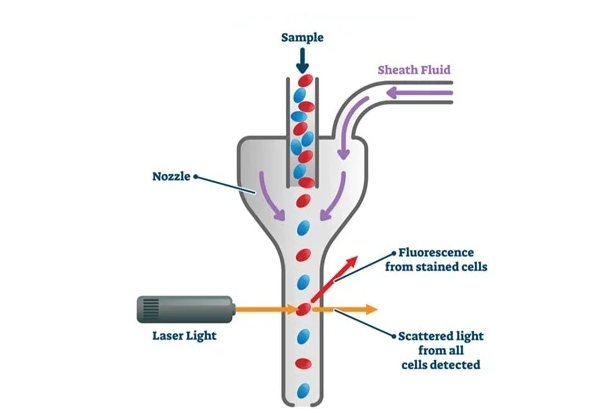
\includegraphics[width=0.9\linewidth]{img/hydro.png}
  \caption{Simplified flow cytometer schema[\url{https://www.shutterstock.com/}].}
  \label{fig:cytm}
\end{figure}

To estimate physical properties of the cell such as size and granularity we take advantage of \emph{light scattering} --- the phenomenon where photons are forced to change their direction by the medium they pass through\cite{scatter98}.

There are two types of scattering measured in cytometry \cref{fig:scatter}.

\emph{Forward scatter} - also referred to as \emph{FSC} or \emph{FSc},  refers to the light, with unchanged wavelength from the source, diffracted around the cell edges - this diffraction pattern roughly corresponds to the cells circumference. 

\emph{Side scatter} - also referred to as \emph{SSC} or \emph{SSc}, is a term used for the light scattered by the cell and its internal structures in the $\geq90^{\circ}$ angle --- this measurement serves as an approximation of cell granularity\cite{fundcyto2011bake}.
\begin{figure}
  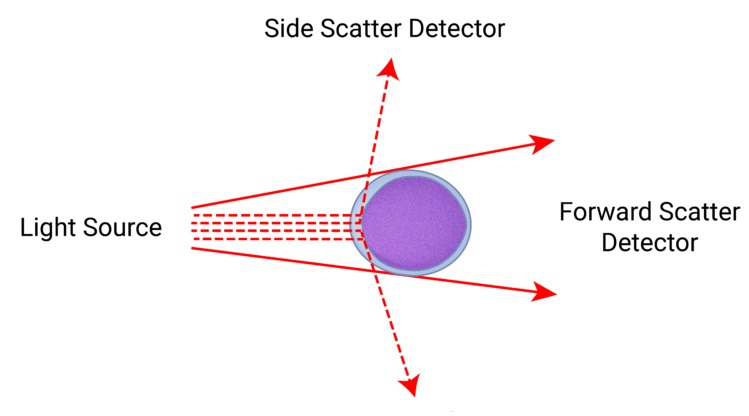
\includegraphics[width=0.65\linewidth]{img/ssc_fsc.jpg}
  \caption{Light scatter pattern for a cell in a cytometer[\url{https://www.learnhaem.com/courses/flow-cytometry/}]}
  \label{fig:scatter}
\end{figure}

In practice FSC and SSC can be used to distinguish cells of interest from cell debris and erythrocytes and furher distinguish broader cell types such as  lymphocytes, monocytes and granulocytes from each other: \cref{fig:gates} A. 

\begin{figure}
  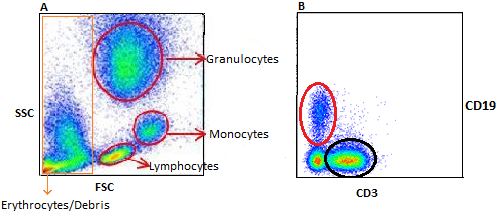
\includegraphics[width=0.75\linewidth]{img/gating.png}
  \caption{A) High-level cell type identification using FSC/SSC plot. B) Separating B (red) and T (black) cells using CD3/CD19 markers.}
  \label{fig:gates}
\end{figure}

To detect biological \emph{markers} such as proteins, we use \emph{antibodies} for the markers we wish to study and \emph{conjugate} them with a distinct \emph{fluorochrome}. 

For each \emph{fluorochrome} absorption and emission spectrum exists. 

Absorption spectrum is the wavelength range at which the fluorochrome can be excited, while the emission spectrum is the range at which it emits photons. 

The emitted light will always have longer wavelength than the absorbed light - this difference is called “Stokes shift”: \cref{fig:stokes}. Higher Stokes shift makes increases  the separation between excitation and emission spectrum easier.

In the context of this thesis, light of 320--808nm wavelength will be considered the main excitation source.

Conjugated antibodies bind to the marker of interest and since the bound fluorochrome emits a specific light spectrum when excited\footnote{\url{https://www.britannica.com/science/fluorescence}} this will alter the \emph{emission spectrum} of the cell.

Thanks to this process we can use a cytometer to measure the cell emission spectrum and later use computational methods and statistical analysis to \emph{unmix} and interpret the data which ultimately allows us to quantify the expression of the studied markers in our cell sample.

\Cref{fig:gates} B illustrates how a marker combination can be used to distinguish cell types and sub-types.

\begin{figure}
  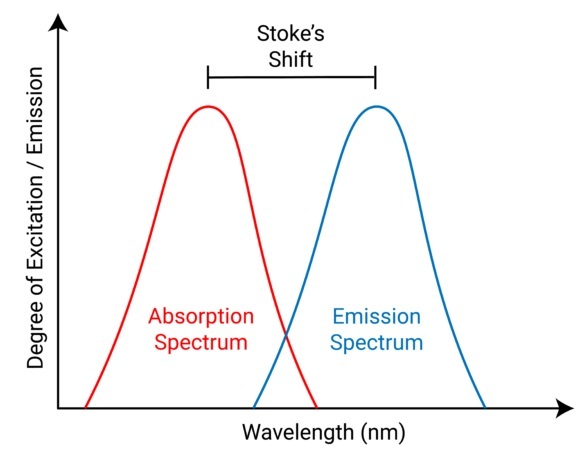
\includegraphics[width=0.5\linewidth]{img/stokes.jpg}
  \caption{Stokes shift [Image taken from Wikipedia article `Stokes shift']}
  \label{fig:stokes}
\end{figure}

It is also important to note that while a fluorochrome can be excited by a light source anywhere within its absorption spectrum, there is an optimal wavelength at which it will absorb the highest fraction of photons, maximizing subsequent emission. This wavelength is called maximal absorbance and the corresponding emission wavelength is called maximal emission. When excited outside of the maximal absorbance wavelength absorption efficiency is relatively decreased\footnote{\url{https://www.olympus-lifescience.com/en/microscope-resource/primer/lightandcolor/fluoroexcitation/}}.

The measured spectrum usually results from combination of the various bound conjugated antibodies and autofluorescence. We can also measure autofluorescence alone on unstained cells where no conjugated antibodies are present in the sample. 

In spectral flow cytometry we need to measure single stain controls - cells with just a single conjugated antibody bound, for every unique fluorochrome used in the current experiment. This is the source of the mixing matrix used for spectral unmixing\cite{mixmat}. 

Spectral flow cytometry leverages multiple lasers with different wavelengths and detector arrays to measure the entire spectrum across a specified wavelength range which is achieved by using a detector array with filters where every detector measures only a narrow part of the spectrum with typical band width of $5-50nm$ that passes through the appropriate filter.\cite{ctyoovw} 

This approach allows using many fluorochromes in a single experiment (up to $\sim 40$  color panels) in turn allowing for more complex cell profiling\cite{40OMIP2020}.

\section{Mixing and spillover}
\label{subs:mixing}

When measuring experiments using more than a few fluorochromes it is practically unavoidable for the respective emission spectra to overlap, meaning that multiple fluorochromes will activate the same detector for the same cell. This phenomenon is called \emph{spillover}.

The main drawback and challenge of spectral cytometry is the need to perform spectral unmixing to infer in what abundances were the fluorochromes originally mixed to produce the measured cell spectrum\cite{unmix2013nonsq}.
In a perfect world where the only noise we have to consider is gaussian and constant this seems to be a linear problem:
\begin{equation}
 y=Mx+r
 \label{eq:base}
\end{equation}

In \cref{eq:base} $y$ is the observation vector (measured spectrum) and $M=D \cdot f$ is a matrix of \emph{spectral signatures} for each of the fluorochromes used in the given experiment. $f$ represents rows of $M$ corresponding to unique fluorochromes used in the experiment while $D$ represents column corresponding to the detectors. $x$ is a vector of fluorochrome abundances and $r$ represents the discussed gaussian noise.\cite{unmix2013nonsq}

While the \emph{mixing matrix} $M$ is not known, it can be estimated using the single stain controls mentioned in \cref{subs:basic}. 

We assume that in any single experiment the number of detectors is higher than the number of fluorochromes, which typically holds true in the real world and leaves us with an overdetermined system of linear equations (more equations than unknowns) solution for which can be estimated using ordinary least-squares\cite{anton2005elementary}. 

A simplified practical example is outlined in \cref{chap:math}.

\section{Noise sources and characteristics}
There are multiple sources of noise in spectral flow cytometry such as staining related deviations, observed population inhomogeneity, electronic noise, noise originating from scattered light not properly excluded by the filters, dark current on photon detectors and noise from photon statistics - a stochastic process influencing both photon emission and detection \cite{noise1985}. 

Combination of the above factors makes the unmixing problem significantly more complicated than it might initially seem.

\subsection{Background noise}
Background noise can be characterized as combination of dark current, optical noise and electronic noise. Dark current is current flowing through a photon detector even without presence of photons. It is caused mainly by thermionic emission\cite{FlCytEl04}.
Optical noise is caused by stray light produced as a result of laser light scattering\cite{PosNoiseSteen92}.

Electronic noise can have many sources such as electromagnetic radiation produced by other electronic devices or other electronic components within the cytometer itself, heat and potentially even gamma rays and x-rays however, those are unlikely to be present in meaningful quantities.

Background noise is relatively independent on current signal. Since it is somewhat constant and relatively low, it can be measured and thresholded against minimizing its impact\cite{FlCytEl04}.
\subsection{Autofluorescence}
Autofluorescence acts as another source of noise with characteristics dependent on the particular cell. It is caused by various compounds and structures inside the cell, such as collagen, elastin, cyclic compounds (commonly pyridine nucleotides) and flavins \cite{af1}\cite{af2}. In mammalian cells the typical excitation range for aurofluorescence lies between 375 to $\sim$640 nm and its typical emission range between $\sim$400 to $\sim$700+ nm\cite{af_ranges}. 

Autofluorescence can be used for unmixing as another spectrum in the mixing matrix $M$, as well as subtracted from the single stain control spectra and the spectra of measured cells prior to unmixing\footnote{\url{https://www.thermofisher.com/cz/en/home/life-science/cell-analysis/flow-cytometry/flow-cytometry-learning-center/flow-cytometry-resource-library/flow-cytometry-methods/spectral-flow-cytometry-fundamentals.html}}. 


When accounted for in unmixing we are effectively negating the noise coming from varition in Autofluorescence strength --- if one cell has 2$\times$ the amount of Autofluorescence as another this is no longer noise instead it becomes an abundance for the Autofluorescence spectrum for that cell in the unmixed data. This effectively helps us lower the amount of noise from Autofluorescence that remains in the data. It now only stems from variations in the shape of Autofluorescence spectrum for individual cells but no longer from its intensity\footnotemark[3]. 

\newpage
\subsection{Poisson (shot) noise}
Poissonian characteristics of photon emission are given by the particle-like nature of light.
The quanta representing photon particles fluctuate in time and these fluctuations can only have discrete values.
This process is best modelled using Poisson distribution function where $\lambda$ is the expected value for number of emitted photons per unit of time\cite{MandelPoisStat1959}.
\begin{figure}
  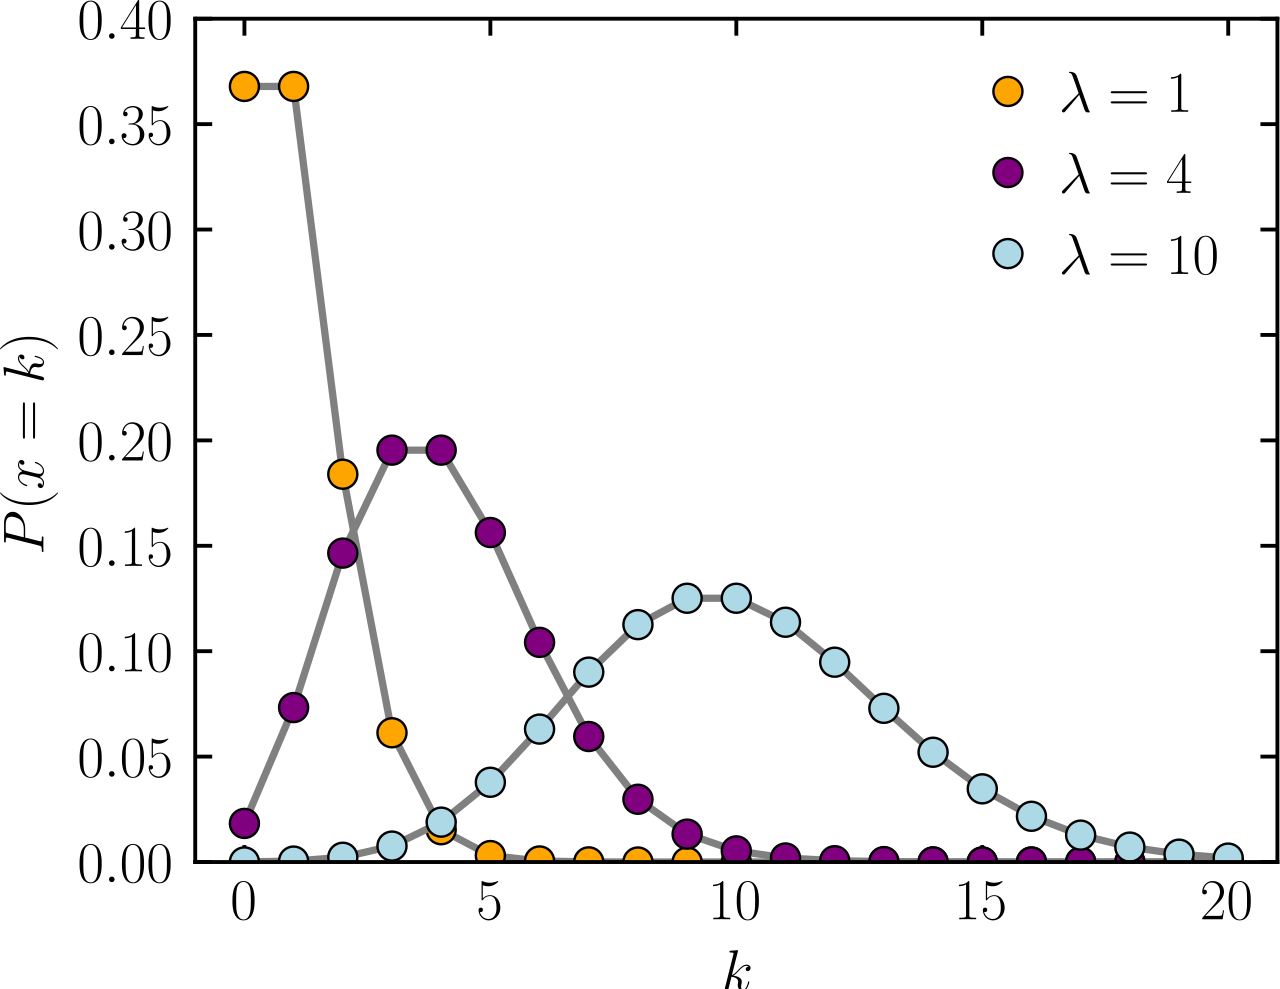
\includegraphics[width=0.7\linewidth]{img/poisson.png}
  \caption{Poisson probability distribution($\lambda=(1,4,10)$) [From Wikipedia.com article `Poisson distribution'].}
  \label{fig:pois}
\end{figure}
 With increasing $\lambda$ the Poisson distribution becomes more and more similar to binomial distribution eventually approximating continuous gamma distribution and finally with high enough $\lambda$ we can say that Poisson distribution approximates normal distribution as seen in \cref{fig:pois}.

There are multiple sources of Poisson noise in spectral flow cytometry:
\begin{itemize}
    \item \emph{Bias light shot noise}
    
    Poissonian noise resulting from background light - this noise should be independent of the current signal level however, it is dependent on the particular optical system (cytometer)\cite{PosNoiseSteen92}. 
    It can also be considered a part of background noise for simplicity.
    
    Assuming that the optical system is in a relatively stable and controlled environment this noise should be constant and can be thresholded against as a part of background noise.
    
    \item \emph{Expression and luminance based noise}
    
    Expression based noise dependens on total expression of targeted proteins by the measured cell. 
    The more targets are expressed, the more conjugated antibodies are going to bind inside the cell. This in turn leads to more internal light scattering, diffraction and interference resulting in higher noise\cite{noise1985}. This noise is unavoidable on real cells that express any of the targets.
    
    Luminance based noise depends on the magnitude of the fluorescent light or fluorescent power --- the integral of the measured cell spectrum. This noise increases across all detectors with rising total fluorescent power making it more significant in dim and less significant in bright detectors\cite{PosNoiseSteen92}. 
    Since this is the signal we want to measure it is also unavoidable. 
\end{itemize}
\chapter{Unmixing methods}
\label{chap:math}
\section{Linear unmixing}
Linear unmixing methods aim to solve the Least Squares problem --- finding the coefficients (abundances in our context) that minimize the squared error between the product of mixing matrix $M$ and abundaces $x$ and the recorded response (emission spectrum of the cell) $y$.

This problem can be optimally solved by multiplying inverse of $M$ by $y$. However this process is strictly linear and rigid --- we cannot introduce any constraints such as non-negative abundance values. 
In spectral flow cytometry, when the previously discussed unavoidable noise sources are introduced this linear solution becomes sub-optimal.
The fact that added noise is not completely random but rather correlated with expression magnitude and total energy of cell emission coupled with the algorithm's inability to respect the non-negativity constraint can lead to wildly inaccurate results. 

\subsection{Trivial zero-noise unmixing example} \label{Unmixing example}
In order to understand the unmixing problem let us first consider a simple example where noise does not exist and we are using a 3-detector system with a 2 fluorochrome panel to unmix spectra measured for a single cell:
M is $f \cdot D$ matrix where $f=2$ and $D=3$ with arbitrarily chosen band values for each fluorochrome spectrum:

\[
M=\begin{bmatrix}
1 & 2 & 3\\
2 & 1 & 1
\end{bmatrix}
\]

$y=\left[7;5;6\right]$ is a vector of length $D$ representing observed spectra of the cell produced by sum of the fluorochrome spectra with abundances $x_1=1$ and $x_2=3$.
This leads to an overdetermined system of equations:
\[\begin{aligned} 
y_1=x_1 M_{\left[1,1\right]}+x_2 M_{\left[2,1\right]} \\ 
y_2=x_1 M_{\left[1,2\right]}+x_2 M_{\left[2,2\right]} \\ 
y_3=x_1 M_{\left[1,3\right]}+x_2 M_{\left[2,3\right]}
\end{aligned}\]
When we substitute known numerical values:
\[\begin{aligned} 
7=x_1 1+x_2 2 \\ 
5=x_1 2+x_2 1\\ 
6=x_1 3+x_2 1
\end{aligned}\]
The solution is then available using only 2 out of the 3 equations:
\[\begin{aligned} 
\text{(row 2)}-2\times\text{(row 1)} &\implies x_2=3 \\
7=x_1+6&\implies x_1=1
\end{aligned}\]
This example illustrates that the naive version of the problem has a trivial solution. 
However, when we introduce noise to the system (which in cytometry is unavoidable and has multiple sources as mentioned previously) it becomes inconsistent and the solution is no longer as simple.

\subsection{Ordinary least squares}
\label{subs:ols}
 This approach minimizes the sum of squared differences between a vector given by multiplying mixing matrix $M$ by abundances $x$ and a vector from measured emission matrix $y$. The formula is given by \cref{eq:ols_standard} and in matrix notation by \cref{eq:ols_mtx}.
\begin{equation}
\underset{x\in R}{\min}{\left\{\sum_{i=1}^{D}\left(y_i-\sum_{k=1}^{f}{x_k M\left[k:i\right]}\right)\right\}}
\label{eq:ols_standard}
\end{equation}
\begin{equation}
\underset{x\in R}{\min}{||Mx-y^2||}
\label{eq:ols_mtx}
\end{equation}
While solution is given by \cref{eq:ols_sol}.
\begin{equation}
M^TMx=M^Ty\ \rightarrow\ x=\left(M^TM\right)^{-1}M^Ty
\label{eq:ols_sol}
\end{equation}
It is important to note that unless $f=D$, $M$ is not a square matrix and therefore neither the term $M^TM$ or $M$ alone is invertible. As mentioned in \cref{subs:mixing} for the purpose of this thesis, the number of fluorochromes in the given experiment will always be lower than the number of dectectors in the optical system used to measure the cell spectra.

We claim that every linear system $Mx=y$ where $M$ is a $f\times D$ matrix has an unique least-squares solution $\hat{x}$.\cite{gallier2020algebra} This holds true because when we interpret $y$ as a point in Euclidean space $R^f$ and column space of $M$ as a subspace $C$ of $R^f$ then $x$ minimizes $||Mx-y^2||$ only if $Mx$ is the orthogonal projection $p$ of $y$ on subspace $R^p$. Which means that $py=y-M\alpha$ and $py\bot C$ (all column vectors of $M\bot C$). Furthermore, if $C^\bot$ is a vector space orthogonal to $C$ then space $x+C^\bot$ intersects $C$ in a point $p$.

It also holds that for any point $x\in C,\ \ px\bot py\rightarrow({xy)}^2=\left(py\right)^2+\left(px\right)^2$. From this Pythagorean relationship it is obvious that $p\in C$ is unique and minimizes distance from $y$ to $C$.

We can express every $x\in\ R^L$ as $x=u+v,\ v\in{\textsc{NullSpace}\left(M\right)}^\bot,\ u\in \textsc{NullSpace}\left(M\right)\rightarrow Mu=0\rightarrow Mx=p$ only if $Mv=p$ . Also because $u\bot v\rightarrow{\ x}^2=u^2+v^2$.

Above proves the existence of unique $x\in{\textsc{NullSpace}\left(M\right)}^\bot$ of minimum norm (if we forfeit the minimum norm condition $x$ no longer has to be unique) that minimizes $||Mx-y^2||$. 

We can then use Moore-Penrose inverse to find minimum norm $\hat{x}$ calculated via singular value decomposition.\cite{gallier2020algebra}

For $n\times m$ matrix $M$ $SVD$ is $M=VDU^T$ where $U$ and $V$ are $n\times n$ and $m\times m$ unitary matrices with columns $\left\{a_1,\ldots,a_n\right\}$ and  $\left\{b_1,\ldots,b_m\right\}$, while $D$ is a diagonal matrix comprising of singular values of $M$. The number of singular values $\left(s_1,\ldots,s_i\right)$ is given by (column) rank of $M$. For $D$, $S$ is $y\times r$ of the singular matrices and the rest is filled with zeros: \cref{eq:svd_D}.
\begin{equation}
D=\left[\begin{matrix}S&0\\0&0\\\end{matrix}\right]
\label{eq:svd_D}
\end{equation}\\
$SVD$ for $M$ can be represented via \cref{eq:svd}.
\begin{equation}
M=\sum_{i=1}^{r}s_ib_i{\vec{a}}_i^t
\label{eq:svd}
\end{equation}
While the pseudo-inverse is given by $M^+=UD^+V^T$ where for $D^+$ \cref{eq:svd_D+}
\begin{equation}
D^+=\left[\begin{matrix}S^{-1}&0\\0&0\\\end{matrix}\right]^\ast
\label{eq:svd_D+}
\end{equation}
And $S^{-1}$ is an $y\times y$ matrix but with inverted singular values of $M \left(s_i^{-1}\right)$  along the diagonals. This corresponds to \cref{eq:svd_pdi}.
\begin{equation}
M^+=\sum_{i=1}^{r}s_i^{-1}b_i{\vec{a}}_i^t
\label{eq:svd_pdi}
\end{equation}
It can be further proven that $M^+$ truly satisfies Penrose conditions and that $M^+$ is Hermitian.\cite{gallier2020algebra}
Pseudo-inverse therefore gives us an efficient and robust way to compute the optimal least squares solution to our problem for minimum norm $\hat{x}\ \rightarrow x^+=M^+y$.\cite{gallier2020algebra}

While this approach provides a solution it is likely to contain negative abundances for some of the fluorochrome spectra  which violates the laws of physics - neither negative photon emission or negative fluorochrome concentration is possible, and will always lead to \emph{spreading} - a phenomenon where the population is distorted and spread along one of the axes, for lower intensity populations.\cite{unmix2013nonsq}

\subsubsection{Ordinary least squares unmixing example}
Expanding on the example from \ref{Unmixing example}. We are using the previously determined system with 3 detectors and 2 fluorochromes.
In R: \begin{lstlisting}[language=r]
spectra=data.frame(D_1=c(1,2),D_2=c(2,1),D_3=c(3,1))
\end{lstlisting}
We are also again simulating a single cell with abundances of  $x_1=1\ ;\ x_2=3$ leaving us with the emission spectrum of $C=\begin{bmatrix}7 & 5 & 6\end{bmatrix}$

In R:
\begin{lstlisting}[language=r]
cell_emitted=spectra[1,]*1+spectra[2,]*3
\end{lstlisting}

While in reality there are multiple noise sources (as discussed) in this simplified example we only consider the noise on detection which we simply model as Gaussian with 0 mean and standard deviation scaled by the total fluorescent power of the cell: \cref{eq:sc_noise}.
\begin{equation}
SD_{noise_C}=0.1\sqrt{\sum_{i=1}^{D}C_i^2}
\label{eq:sc_noise}
\end{equation}
In R: 
\begin{lstlisting}[language=r]

cell_received=cell_emitted +
rnorm(length(cell_emitted),sd=0.1*sqrt(sum(cell_emitted^2)))
\end{lstlisting}
This simulates the fact that in dimmer detectors the brightness variability given by Poissonian characteristics of photon emission is going to be proportionally higher than in bright detectors resulting in higher relative noise. 

Finally we use \texttt{lm()} function in R that fits a linear regression model via OLS using SVD and Moore-Penrose inverse:
\begin{lstlisting}[language=r]
lm(t(cell_received)~t(spectra)+0)
\end{lstlisting}
Note that we are setting the intercept to 0, since we assume that if the received spectrum is 0 then all abundances should also be 0.

Resulting abundances after OLS unmixing are $x_1=0.9216\ ;\ x_2=2.8491$. These coefficients are obviously dependent on the exact noise values that are randomly sampled, therefore the result will differ depending on set random seed state.

Since the standard deviation for out noise model is scaled by the total fluorescent power of the measured spectra (integral of intensity across all detectors) on average the absolute noise in every detector is the same however, relative noise increases with decreasing fluorescent power resulting in noisier dim parts of the spectra. This corresponds to the discussed characteristics of real world detectors and will later be useful for generating artificial testing data.

It would be appropriate to reiterate on the main advantage of OLS. As we have shown in \cref{subs:ols} pseudoinverse matrix needed to solve OLS problem can be computed using singular value decomposition and matrix operations. Using modern computers these operations can be performed extremely quickly making OLS lightning fast even for very large datasets (millions of cells). The \texttt{pinv} function from \texttt{R} package \texttt{pracma} computes Moore-Penrose generalized inverse (pseudoinverse) of matrix $A$ denoted as $B$ via $\text{SVD}$ that can be then used to minimize $|A x - b|$ by setting $x = B b$. In R\footnote{\url{https://www.rdocumentation.org/packages/pracma/versions/1.9.9/topics/pinv}}:

\begin{listing}
\begin{lstinputlisting}[language=r]{misc/pracma_pinv_commented.R}
\end{lstinputlisting}
\caption{A commented version of \texttt{pinv} function from R library \texttt{pracma}, used to compute matrix pseudoinverses. The result can be used to perform OLS unmixing, as described in \cref{subs:ols}}
\label{lst:ex}
\end{listing}

On any remotely modern system this computation is very fast even for hundreds of thousands of cells (~6 seconds for one million cells when tested on a single core of a Ryzen 9 5900X cpu). 

However, with constantly increasing performance of consumer-grade hardware and the advent of GPU acclerated computing even much more expensive methods such as gradient descent based algorithms become viable even for very large data.

\subsection{Weighted least squares}
WLS approach takes into consideration noise variance growing with increasing signal intensity. It does this without modelling the dual Poissonian process responsible. Instead it uses weights for the mixing matrix that are inversely proportional to the signal strength. In place of squared error this approach minimizes the mean absolute percentage error (MAPE) defined as \cref{eq:MAPE}.
\begin{equation}
\text{MAPE}=\frac{100}{n}\sum_{i=1}^{n}|\frac{x_i-y_i}{x_i}|
\label{eq:MAPE}
\end{equation}
For WLS spectral unmixing this can be expressed as in\cref{eq:wls_x}\cite{unmix2013nonsq} 
\begin{equation}
E_p=j^T|(y-Mx)|\circ\bar{y}
\label{eq:wls_x}
\end{equation}
\begin{equation}
\hat{x}=(M^TW^2M)^{-1}M^TW^2y
\label{eq:ols_x}
\end{equation}
We can solve for $\hat{x}$ directly using \cref{eq:wls_x}.

This above equation becomes the solution for the OLS unmixing problem when $W$ is an identity matrix. To solve for WLS $W$ is set in inverse proportion to the signal strength\cite{unmix2013nonsq}.

While this approach works well for rudimentary simulated data it was shown not perform optimally for real data where it tends to distort populations and produce negative abundance values even more so than OLS\cite{unmix2013nonsq}.


\section{Non-linear approaches to unmixing}

The non-linear approaches to spectral unmixing may take into account the previously discussed spillover spreading and multiple scattering --- scattering of light that occurs in different parts of the cell and the interaction between resulting scatters. As alluded to before, in spectral flow cytometry this phenomenon manifests in variation that is non-linearly dependent on fluorescent power and expression magnitude. This fact makes dim populations noisier and harder to unmix using only linear models.

Another problem this method could help with, is the error produced when measuring spectra for unmixing from single stain controls - dimmer parts of the spectra measured for the mixing matrix $M$ are less accurate as well.

Combination of these factors suggests that a non-linear iterative method ideally with a customizable weighting option has a potential to perform better than linear methods such as OLS. 

\subsection{Non-negative ordinary least squares}
This is a modification of the OLS approach where $\alpha$ is constrained to non-negative values ($\alpha_i\geq0$) with additional condition stating that unmixed abundances must sum to $100\%$ of the observed vector $y$.\cite{unmix2013nonsq}

It is important to note that this modification of ordinary least squares cannot be computed using the pseudo-inverse and instead is computed using NNLS iterative algorithm from \cite{Bro1997AFN}.
While this approach is not equivalent to using ordinary least squares and setting all negative abundances to 0, in practical applications the results are similar. The populations are clipped and data points pile up on the axes.\cite{unmix2013nonsq}

\subsection{Utilizing gradient descent for unmixing}
\begin{equation}
y=\sum_{i=1}^f x_iM_{i*}+r
\label{eq:base_ext}
\end{equation}
We can express the main mixing hypothesis from \cref{eq:base} as \cref{eq:base_ext} where $y$ is the observed fluorescence vector of length $D$ (given by the number of detectors in the experiment) for the given cell and $M=f \cdot D$ is the mixing matrix with $f$ being the number of fluorochromes used. 
Parameters $x_{1,...,f}$ represents the abundances for fluorochromes $M_{1*},...,M_{f*}$ corresponding to rows of the mixing matrix $M$ and $r$ represents noise.
\subsubsection{Cost function}
Our goal then becomes to minimize the cost function given by \cref{eq:sq_err}.
\begin{equation}
C(x)=\frac{1}{2D}\sum_{j=1}^{D}(y_{p_j}-y_{o_j})^2
\label{eq:sq_err}
\end{equation}

Constant $\frac{1}{2}$ is used to get a cleaner derivative and does not affect the minimization in any way. The cost function represents mean of squared difference between the predicted cell vector $y_p$ - calculated as the product of unmixed abundances and respective spectra from the measured mixing matrix, and the observed cell vector $y_o$.

Thanks to the convex nature of this function there is no risk of getting stuck in a local minimum as demonstrated in \cref{fig:gdp}.

\begin{figure}
  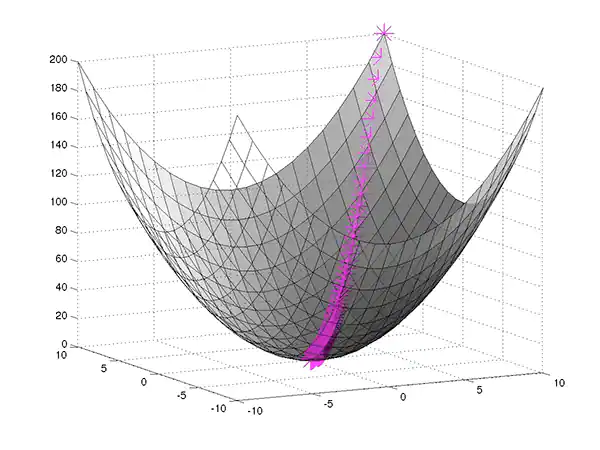
\includegraphics[width=100mm]{img/gdpic.png}
  \caption[]%
  {Gradient descent on 3D convex function [\url{https://www.digikey.be/nl/articles/get-started-machine-learning-hardware-and-software}].}
  \label{fig:gdp}
\end{figure}

\subsection{General gradient descent algorithm}
This section outlines the iterative process of calculating gradient descent for the objective function (MSE) we aim to minimize:

\begin{enumerate}
  \item \textbf{Compute gradient.}
  Calculate the first order partial derivative of the cost function with respect to each of the parameters.
  \item \textbf{Step in the opposite direction} 
  Subtract the gradient scaled by learning rate from parameter value.
  \item \textbf{Repeat until stop condition} Repeat the process until preset stop condition (or one of multiple) is reached.
\end{enumerate}

When we extend the example from \cref{Unmixing example}.
   We need to compute the gradient of the error function specific to our example from \cref{eq:err_gd_spec} in order to obtain the slope of tangent touching the error function with respect to the given parameter.
  \begin{equation}
  \frac{\partial}{\partial x_i} C(x)=\frac{\partial}{\partial x_i}\frac{1}{2D}\sum_{j=1}^{D}(\sum_{i=1}^{f}(x_iM_{i,j})-y_j)^2 
  \label{eq:err_gd_spec}
  \end{equation}
Substituting in:
  \[\begin{aligned}
  \frac{\partial}{\partial x_i} C(x)=\frac{\partial}{\partial x_i}\frac{1}{2D}(&(x_1 M_{1,1}+x_2 M_{2,1}-y_1)^2\\
  +&(x_1 M_{1,2}+x_2 M_{2,2}-y_2)^2\\
  +&(x_1 M_{1,3}+\alpha_2 M_{2,3}-y_3)^2)
 \end{aligned}\]

 If we take the partial derivative with respect to $x_1$ (partial derivative with respect to $x_2$ can be computed analogically):

  \[\begin{aligned}
  \frac{\partial}{\partial x_1} C(x)=&M_{1,1}(x_1 M_{1,1}+x_2 M_{2,1}-y_1)\\
  +&M_{1,2}(x_1 M_{1,2}+x_2 M_{2,2}-y_2)\\
  +&M_{1,3}(x_1 M_{1,3}+x_2 M_{2,3}-y_3)
 \end{aligned}\]
 Let us assume that from previous parameter update our current abundances are $x_1=0.9$ and $x_2=2$. We can now compute the gradient (analogically for $x_2$):
  \[\begin{aligned}
  \frac{\partial}{\partial x_1} C(x,t)=&1(0.9 \cdot 1+2 \cdot 2-7)\\
  +&2(0.9 \cdot 2+2 \cdot 1-5)\\
  +&3(0.9 \cdot 3+2 \cdot 1-6)\\
  =&-8.4
 \end{aligned}\]
  Next we use the the computed gradient for parameter update: \cref{eq:gd_update}. By subtracting the gradient we are stepping against it and therefore towards the minimum of the cost function.
 \begin{equation}
 x_i(t+1)=x_i(t)-\alpha\frac{\partial}{\partial x_i} C(x,t)
 \label{eq:gd_update}
  \end{equation}

 In \cref{eq:gd_update} $x_i(t)$ represents new value for the i-th abundance at current iteration, while $x_i(t)$ is the value from previous iteration. Finally $\alpha$ is the learning rate - a scaling factor (usually $\alpha<<1$) for the step size which needs to be set appropriately --- this means not too high so that gradient descent algorithm is able to converge to the minimum, and not too low in order for convergence to happen in reasonable time.
 
 Gradient from our example is negative which results in parameter increment. The increment magnitude will depend on learning rate and gradient size.
 
 We repeat the parameter update until we reach a predefined stop condition. While in an ideal world this would be 0 gradient (which corresponds to 0 sum of residuals), in real world this unlikely to ever happen. This is why we selected maximum number of iterations as our stop condition.
 
 However our example is idealized and we should be able to reach $100\%$ accurate abundances via a reasonable number of gradient descent iterations. When this happens and we recalculate the gradient with abundances $x_1=1$ and $x_2=3$:

  \[\begin{aligned}
  \frac{\partial}{\partial x_1} C(x,t)=&1(1 \cdot 1+3 \cdot 2-7)\\
  +&2(1 \cdot 2+3 \cdot 1-5)\\
  +&3(1\cdot 3+3 \cdot 1-6)\\
  =&0
 \end{aligned}\]
Indeed the gradient is 0 as expected. 


\subsection{Gradient descent variants implemented in Nougad}
Nougad is a library designed for the purpose of spectral unmixing, efficiently implemented in $C$ programming language with $R$ language interface \footnote{\url{https://github.com/exaexa/nougad}}. 
\subsubsection{Nougad variation on momentum method}
Momentum-based modification of the gradient descent algorithm "remembers" the previous update and allows it to increase the magnitude of the current update if they are both moving in the same direction. An acceleration factor is introduced to scale the influence of the previous update.

\begin{algorithm}
\caption{Nougad parameter update}
\label{algo:ngd_moment}
\begin{algorithmic}
\State $it \gets 0$
\While{$true$}
    \If{$up_i(t-1)\frac{\partial}{\partial x_i} C(x,t) > 0$} 
        \State $up_i(t) = \gamma up_i(t-1)+\frac{\partial}{\partial x_i} C(x,t)$
    \Else
        \State $up_i(t) = \frac{\partial}{\partial x_i} C(x,t)$
    \EndIf 

    \State $x_i(t) = x_i(t-1)+\alpha up_i(t)$
    \State $it = it+1$
    \If{$it \geq maxit$}
        \State $break$
    \EndIf 
\EndWhile
\end{algorithmic}
\end{algorithm}


In \cref{algo:ngd_moment} $\gamma$ represents the acceleration parameter while $up_i(t)$ is the update for $i$-th parameter in time $t$ and $maxit$ the number of iterations after which the algorithm stops.

Nougad also adds three options that are important in the context of spectral unmixing. 
\begin{enumerate}
    \item \emph{Contribution of negative abundances. - \param{nw}}
    
    This option sets a scaling factor for the contribution of negative spectral abundances to the update.
    Since we know that negative spectral abundances are impossible this parameter allows us to set a bias against such results.
    \item \emph{Contribution of positive/negative residuals - \param{spw}/\param{snw}}
    
    This option allows us to set a factor by which positive and negative residuals contribute to gradient, allowing us to set a preference for either positive or negative residuals and magnitude of their influence.
    \item \emph{Starting abundances - \param{start}}
    
    This option allows us to set a starting position for all abundances. Instead of starting at 0 we can potentially start at a number closer to a median value of the real abundances and hypothetically decrease the number of iterations needed to reach a solid result.
\end{enumerate}

Note that weighting the residuals and spectral abundances using \param{spw}, \param{snw} and \param{nw} is not considered in this pseudo-code to make it more concise however, it is a simple multiplication by a scalar. This implementation further allows us to explicitly set all other parameters used in gradient descent calculation including learning rate \param{alpha ($\alpha$)}, acceleration factor \param{accel ($\gamma$)} and a number of iterations \param{maxit}.

\subsubsection{Adam version of Nougad}
Adam stands for Adaptive Moment Estimation. The method computes the update based on moving averages of both the gradient itself (first moment) and its square (second moment), each with its own acceleration factor. 

\begin{equation}
\begin{aligned}
m_a(x_i,t) &= \beta_1 m_a(x_i,t-1)+(1-\beta_1)\nabla_iC(x)\\
m_s(x_i,t) &= \beta_2 m_s(x_i,t-1)+(1-\beta_2)\nabla_i^2C(x)\\
x_i(t) &= x_i(t-1)+\alpha \frac{m_a(x_i,t)}{\sqrt{m_s(x_i,t)}+\epsilon}
\end{aligned}
\label{eq:adam}
\end{equation}



In \cref{eq:adam} \param{b1 ($\beta_1$)} and \param{b2 ($\beta_2$)} are acceleration factors for first and second moment moving averages and $\epsilon$ is a very small scalar (usually $\leq 10^{-6}$) needed to avoid division by zero.

Options to emphasize influence of negative spectra abundances and positive/negative residuals are kept from the first method. All parameters including desired maximum number of iterations can again be passed as function arguments.
\subsection{Performance and acceleration of nougad}
Base implementation of nougad runs on CPU and is only single-threaded and while is inherently much slower than OLS it is still fast enough for an odd unmixing task. However, for any optimization/testing effort that requires hundreds or thousands of runs on large datasets (such as this thesis) a more performant implementation is desirable.

Luckily, since results of nougad for each cell are completely independent on other cells it lends itself very well to parallelization efforts. Simply put we can split cells into batches depending on core count and process them in parallel. In C we can even leverage pointers to avoid copying any of the large matrices as at no point should two threads process the same element.

A potential parallelized version therefore promises vast (and most likely near-linear) increase in performance for multi-threaded CPUs and potentially even higher performance for a version leveraging modern GPUs.  



\chapter{Evaluating the performance of unmixing algorithms}

Our main goal is to evaluate performance of Nougad algorithm in both its momentum-based and ADAM variants against Ordinary Least Squares (OLS) and Weighted Ordinary Least Squares (WOLS) methods. 

We will also evaluate the performance for all the methods with the unmixing results clamped to zero --- negative abundance values in the unmixing result will be replaced with zeros.

\section{Generating artificial data sets}

To accurately and objectively measure the performance of various unmixing methods it is imperative to have a benchmark data set where ground truth is known. This is of course not possible when it comes to real world experiments since it is impossible to obtain ground truth abundances --- that is the reason are trying to find a better unmixing algorithm.

When generating such artificial data we should try to model the processes responsible for spectra emission and detection as accurately as possible while still keeping the model reasonably simple.

Note that we are generating Lymphocyte-like cells and their various sub-types only as this should be sufficient for testing purposes. However, if required it is easy to extend the phenotype table by additional cell types such as Monocytes.

The code responsible for generating the artificial data is available in supplementary materials as well as on Github\footnote{\url{https://github.com/mattejn/artificial_data_comp}}.

The general step-by-step process for generating artificial data is: 
\begin{enumerate}
\item{Obtain spectra for different fluorochromes.}
\item{Obtain phenotype characterizations for simulated cells.}
\item{Generate a fraction of dead cells for each phenotype}
\item{Simulate expression variability.}
\item{Simulate expression dependent noise.}
\item{Calculate cell emission spectra.}
\item{Simulate brightness-dependent noise.}
\end{enumerate}
  \subsection{Obtaining spectra for different fluorochromes} 
  Spectra can be either artificially generated and arbitrary or measured from single stain controls of a real experiment.  We decided to go with the latter to hopefully make the model more realistic however, this does not necessarily make the former approach less valid. The spectra was measured using the \texttt{R} application \texttt{PanelBuildeR} \footnote{\url{https://github.com/exaexa/panelbuilder}}.
  
  Either way the spectra form a standard unmixing matrix $M=D \cdot f$. Condition that states that there must be more individual detectors used for measurements than the number of distinct fluorochromes used in the experiment applies.
  
  Each fluorochrome is referred to by the name of the corresponding antibody from the reference real world experiment. 
  
  \subsection{Obtaining phenotype characterizations}
  In our approach phenotype matrix $P$ takes the form of $P=C_t*f$ giving probabilities of each fluorochrome $f$ (columns) for each cell type or sub-type $C_t$ (rows) --- each row in the matrix therefore represents an unique cell type.
  
  Furthermore, each row has a parent column that tells us what previously defined phenotype the current phenotype inherits abundances from. This allows us to only fill only the fluorochrome abundances that are different from the parent and leave the inherited blank, as in \cref{tab:packed_pheno}. 
  
  Relative cell counts for each phenotype are simply given by a vector $c$ of length $C_t$. Note that parent-child relationships are valid even for counts - this means that relative count for a child is a proportion of the parents relative count. 
  



  
\begin{table}
\small\sf
\label{tab:packed_pheno}
\begin{tabular}{lllcccccc}\toprule 
\multicolumn{2}{c}{Population}  &  \multirow{2}{3.5em}{Relative count} & \multicolumn{6}{c}{Antigens}\\ 
\cmidrule(l{.5em}r{.5em}){1-2}
\cmidrule(l{.5em}r{.5em}){4-9}
parent & current & {} & CD3 & CD56 & NKG2A  & CD4   & CD8   & AF\\
\midrule
-           & base    & 1             & 0   & 0    & 0      & 0     & 0     & 0  \\
base        & AF      & 0.95          &     &      &        &       &       & 1  \\
AF          & T       & 0.5           & 1   & 0    & 0.0052 & 0.738 & 0.224 &    \\
AF          & NK      & 0.2           & 0   & 1    & 1      & 0     & 0.14  &    \\
AF          & NK T    & 0.1           & 1   & 1    & 0.04   & 0.162 & 0.752 &    \\
T           & CD4     & 0.5           &     &      & 0      & 1     & 0     &    \\
CD4         & Thelper & 0.8           &     &      &        &       &       &   \\
\bottomrule
\end{tabular}
\caption{Example of a packed phenotype table.}
\end{table}


  This tree-like structure is then unpacked using a recursive function (available in the supplement) leaving us with a matrix that defines expression probability of each of the antibody targets for each cell type and their relative count in the resulting data set. $c$ is then normalized to one to give proportions of different phenotypes and multiplied by the desired number of cells for the entire data set giving us the extended probability matrix $Pex$.
  
  A partial example of an unpacked phenotype table with normalized relative counts is available in \cref{tab:unpacked_pheno}.
  
  When created $Pex$ is copied into $PexD$ which will be used to generate dead variations of the simulated cells. Finally $c$ is multiplied by $0.825$ scalar for $Pex$ and $0.175$ scalar for $PexD$ (creating $cd$) respectively - this represents the desired ratio of live ($82.5\%$) and dead ($17.5\%$) cells in the resulting data. This ratio is mostly arbitrary --- we simply wanted our data set to contain some number of dead cells without going overboard. Dead cell ratio can be changed using the appropriate parameter in the generator function or even disabled (set to 0).
  
  Absolute counts are rounded to the nearest integer.
  
\begin{table}\small\sf\
\label{tab:unpacked_pheno}
\begin{tabular}{lllcccccc}\toprule 
\multicolumn{2}{c}{Population}  &  \multirow{2}{3.5em}{Relative count} & \multicolumn{6}{c}{Antigens}\\ 
\cmidrule(l{.5em}r{.5em}){1-2}
\cmidrule(l{.5em}r{.5em}){4-9}
parent & current & {} & CD3 & CD56 & NKG2A  & CD4   & CD8   & AF\\
\midrule
AF          & NK       & 0.19     & 0   & 1    & 1     & 0     & 0.14  & 1  \\
AF          & NK T     & 0.095    & 1   & 1    & 0.04  & 0.162 & 0.752 & 1  \\
Thelper     & resting  & 0.1254   & 1   & 0    & 0     & 1     & 0     & 1  \\
Thelper     & effector & 0.0646   & 1   & 0    & 0     & 1     & 0     & 1  \\
Treg        & resting  & 0.03135  & 1   & 0    & 0     & 1     & 0     & 1  \\
Treg        & effector & 0.01615  & 1   & 0    & 0     & 1     & 0     & 1  \\
CD8         & naive    & 0.095    & 1   & 0    & 0     & 0     & 1     & 1  \\
\bottomrule
\end{tabular}
\caption{Partial example of a probability matrix from unpacked phenotypes.}
\end{table}
  
  \begin{algorithm}
  \caption{Extended probability matrix calculation}
  \label{alg:exprob}
  \begin{algorithmic}
  \State $cd \gets c$
  \State $Pex = []$
  \State $PexD = []$
  \State $a = 0$
  \State $b = 0$
  \For {$ i=1,..,N$}
  \State $c_i = c_i\div \sum{c}$
  \State $c_i = \lceil c_i \cdot m \cdot 0.825 \rfloor$
  \State $cd_i = \lceil c_i \cdot m \cdot 0.175 \rfloor$
  \For{$ k=a,..,(a+c_i$)}
  \State $Pex_{k*} = P_{i*}$
  \EndFor 
  \For{$ k=b,..,(b+cd_i$)}
  \State $PexD_{k*} = P_{i*}$
  \EndFor 
  \State $a = a+c_i$
  \State $b = b+cd_i$
  \EndFor 
  \end{algorithmic}
  \end{algorithm}
  
  \Cref{alg:exprob} is responsible for extended probability matrix calculation where $N$ corresponds to length of $c$ and $m$ to desired number of cells. $Pex$ is therefore given by repeating each row from $P$ times $c_i$ - the appropriate element of $c$. Analogically for $PexD$ and $cd_i/cd$. 
  
  A small example of an extended probability matrix can be found in: \cref{tab:ex_prob}
  

\begin{table}[]\small\sf
\label{tab:ex_prob}
\begin{tabular}{lcccccc} \toprule 
\multirow{2}{*}{Population}  & \multicolumn{6}{c}{Antigens}\\ 
\cmidrule(l{.5em}r{.5em}){2-7}
{} & CD3 & CD56 & NKG2A  & CD4   & CD8   & AF\\
\midrule
AFNK.14          & 0   & 1    & 1     & 0     & 0.14  & 1  \\
AFNK.15          & 0   & 1    & 1     & 0     & 0.14  & 1  \\
AFNK T           & 1   & 1    & 0.04  & 0.162 & 0.752 & 1  \\
AFNK T.1         & 1   & 1    & 0.04  & 0.162 & 0.752 & 1  \\
T helper resting   & 1   & 0    & 0     & 1     & 0     & 1  \\
T helper resting.1 & 1   & 0    & 0     & 1     & 0     & 1  \\
T helper effector  & 1   & 0    & 0     & 1     & 0     & 1 \\
 \bottomrule
\end{tabular}
\caption{Partial example of an extended probability matrix.}
\end{table}
  
  Relative counts and even phenotypes could be randomly generated however, we decided to use a matrix kindly provided by the thesis advisor representing the typical phenotypes for human Lymphocytes and their ratios in a real experiment as this should again lead to a more realistic model.
  
  \subsection{Simulating dead cells}
  In a real world experiment it is very likely that a significant fraction of measured cells ends up somehow damaged or dead as a result of chemical stress, apoptosis, and other causes.
  
  To simulate this fact we have created $PexD$ matrix in the previous step. Expression probabilities in $PexD$ are row-wise (per cell) multiplied by $sd$ - a vector of scalars randomly sampled from 0.3--0.6 range with appropriate length. This vector represents attenuated expression in the damaged cells. 
  
  Furthermore, a column vector $LDd$ is aded to both $Pex$ and $PexD$ representing expression probabilities for `LIVE/DEAD blue' dye. This stain binds to free amines found in cells with a damaged membrane. Probability vector for these amines in $PexD$ is semi-randomly set in 0.6--1 range. 
  
  The semi-randomness stems from the fact that each element of $LDd$ - $LDd_i$ is actually calculated by randomly sampling from 0.3--0.5 range and then adding $1-sd_i$ where $sd_i$ is the appropriate element $sd$. Finally, since the maximum possible value for this formula is actually 1.1 any element $LDd_i>1$ is set to one. 
  
  This results in the 0.6--1 range that is somewhat inversely correlated with expression attenuation (the more attenuated the expression, the more damaged we expect the cell to be, which would lead to more free amines) and slightly biased to higher values.
  \begin{algorithm}
  \caption{Dead phenotypes probability matrix}\label{alg:deadprob}
  \begin{algorithmic}
  \State $nc = ncol(PexD)$
  \State $d = [N]$
  \For {$ i=1,..,N$}
  \State $d_i = RandSamp\langle0.3;0.6\rangle$
  \State $PexD_i = PexD_i \cdot d_i$
  \State $d_i = (1-d_i)+RandSamp\langle0.3;0.5\rangle$
  \If{$d_i>1$}
  \State $d_i=1$
  \EndIf
  \State $PexD_{i(nc+1)}=d_i$
  \State $Pex_{i(nc+1)}=0$
  \EndFor 
  \State $Pfull=\left[ \begin{array} {c} Pex \\ PexD\end{array}\right]$
  \end{algorithmic}
  \end{algorithm}
  Finally $Pex$ and $PexD$ are row-wise joined creating the full probability matrix $Pfull$. For pseudocode refer to \cref{alg:deadprob}.

  
  \subsection{Simulating expression variability}
  Spectral abundances and are generated from the probability matrix leveraging the fact that for real world experiments the positive populations are expected at around $10^4$ mark.
  
  Before generating the abundances we split our column vectors into strong and weak markers. Strong markers have higher abundance floor than weak markers. This means that we need to use different processes to generate abundance values for these subsets. 
  
  \begin{algorithm}
  \caption{Abundances from probabilities}\label{alg:abund}
  \begin{algorithmic}
  \State $u = 1.5$
  \State $s = {2,3,9,14,17,21}$
  \State $D = ncol(Pfull)$
  \For {$ i=1,..,N$}
  \For {$ k=1,..,D$}
  \If {$D \in s$}
  \State $Pfull_{ik}=10^{(4-u)+u\cdot SampBinom(Pfull_{ik})+SampNorm(mean=0,sd=0.2)}$
  \Else
  \State$Pfull_{ik}=10^{2+2\cdot SampBinom(Pfull_{ik})+SampNorm(mean=0,sd=0.2)}$
  \EndIf
  \EndFor 
  \EndFor 
  \State $Ex=Pfull$
  \end{algorithmic}
  \end{algorithm}
  
  To differentiate strong markers we raise the floor from $10^2$ that is set for weak markers to $10^{4-u}$ where $0<u<2$ in order to strengthen strong marker expression. We tested $u=1$ and $u=1.5$ sticking with the latter when generating data for the final evaluation. 
  
  In \cref{alg:abund} $N$ represents the number of rows in the probability matrix $Pfull$ and $D$ number of columns. Function \texttt{SampBinom} samples single value from binomial distribution with the provided probability (current element of $Pfull$) simulating probability-based expression in the current cell for the current conjugated antibody target. Function \texttt{SampNorm} samples a single value from normal distribution with the provided parameters - $\text{mean}=0$ and $\text{standard deviation}=0.2$ simulating natural variability for both "positive" and "zero" expression. 
  
  This process leaves us with Expression matrix $Ex$ with abundances ranging from $\sim 10^2$ to $\sim 10^4$. We consider $Ex$ ground truth - it represents real abundances without noise. The closer the unmixing algorithm can get to those values the better we consider its performance. 
  
  In order to simulate noise resulting from the total amount of conjugated antibodies bound to target proteins we add Gaussian noise with standard deviation proportional to the sum of expression in each cell. The 0.001 scaling factor is only an estimate and can be adjusted within reasonable bounds: \cref{alg:expr_noise}.
  
  \begin{algorithm}
  \caption{Expression based noise}\label{alg:expr_noise}
  \begin{algorithmic}
  \State $N = nrow(Ex)$
  \State $D = ncol(Ex)$
  \For {$ i=1,..,N$}
  \For {$ k=1,..,D$}
  \State $Ex_{ik}=Ex_{ik}+SampNorm(mean=0,sd=(\sum{Ex_{i*}})\cdot 0.001)$
  \EndFor 
  \EndFor 
  \end{algorithmic}
  \end{algorithm}
 
\subsection{Calculating cell emission spectra and noise}
Cell emission spectra are calculated as a matrix product of the abundance matrix $Ex$ and the mixing matrix $M$ giving us the emission matrix $Em$. Each row of $Em$ then represents the resulting emission spectrum of a given cell - gained by multiplying the individual fluorochrome spectra from $M$ by their respective abundances for the given cell and summing the results: \cref{eq:emission}.
\begin{equation}
 Em = Ex \times M 
 \label{eq:emission}
\end{equation}

We are adding zero mean Gaussian noise to each element of $Em$ with standard deviation given by L2 norm of the given cell vector which corresponds to the total energy of the given cell or its fluorescent power. Note that we are using L2 norm because it better corresponds to the signal energy in physics context than L1/Hamming norm used in the case of expression-dependent noise: \cref{alg:power_noise}.

\Cref{fig:2D_gen} illustrates how does adding luminance-based noise affect the data in 2 selected dimensions.

  \begin{algorithm}
  \caption{Fluorescent power based noise}
  \label{alg:power_noise}
  \begin{algorithmic}
  \State $N = nrow(Em)$
  \State $D = ncol(Em)$
  \For {$ i=1,..,N$}
  \For {$ k=1,..,D$}
  \State $Em_{ik}=Em_{ik}+SampNorm(mean=0,sd=(\sum{Em_{i*}^2})\cdot 0.0005)$
  \EndFor 
  \EndFor 
  \end{algorithmic}
  \end{algorithm}
  

 
\begin{figure}
 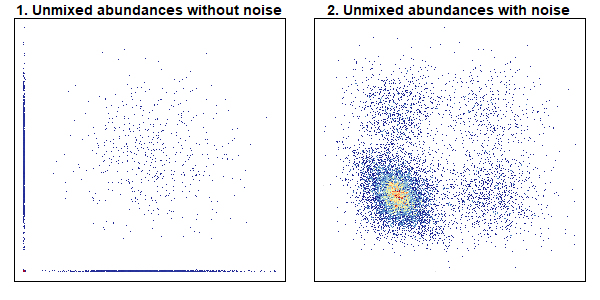
\includegraphics[width=1\linewidth]{img/2D_gen2.png}
 \caption{2D plot illustrating change caused by adding luminance-based noise.}
 \label{fig:2D_gen}
\end{figure}

\section{Nougad hyperparameter optimization}
 
\subsection{Multithread implementation of Nougad}
For the purpose of the hyperparameter optimization a significant speed boost for the Nougad algorithm was needed.

This is why we have modified the original code to allow parallel execution creating a multi-threaded fork of Nougad. Threading support is implemented directly in the $C$ function\footnote{\url{https://github.com/mattejn/nougad_mt}} which was not a trivial task for the author previously completely unfamiliar with $C$ programming language.

We also believe that this version will be helpful to others as vast majority of scientist has access to multi-threaded systems.

The speed improvement is very significant. For one million cells the unmixing time is reduced from $\sim$2 minutes to $\sim$6 seconds on 12 core/24 thread Ryzen 9 5900X CPU representing $\sim$20$\times$ speed increase (and purely by chance taking very similar amount of CPU time as the Moore-Penrose based calculation of OLS - which is of course single-threaded, on the very same CPU). 

Benchmark is available in supplemental materials as well as from Github\footnote{\url{https://github.com/mattejn/artificial_data_comp}} and as a part of the supplemental materials.

Linear performance increase is expected with increase in available CPU resources for single-CPU and most likely even multi-CPU systems.
 
\subsection{Available hyperparameters}
 
 Unlike OLS and WLS, Nougad is a tunable algorithm that gives us the option to influence its performance and behavior by changing its hyperparameters.
 
 Tunable parameters:
 \begin{enumerate}
    \item \emph{Spectra negative/positive weights - \param{snw}/\param{spw} }

    
    These parameters serve to weight the contribution of individual residuals when calculating the gradient, allowing us to set a bias towards/against positive/negative residuals. These scalars get converted to a weighting matrix. 

    \item \emph{Weights of non-negative learning factor - \param{nw}} 

    
    This gets converted to a vector of length $f$ and serves a bias against negative spectral abundances in the results. The higher this parameter is set the higher the cost for negative abundances becomes. It can be set as vector which could potentially be useful if we had a good reason to disproportionately "distrust" some of the spectra in a particular experiment.

    \item \emph{Starting points for gradient descent - \param{start}}

    
    Option that controls the starting points for abundance matrix. Setting this closer to a median abundance value for the unmixed data set could improve performance/reduce the number of iterations needed to reach a good result.

    \item \emph{Learning rate - \param{alpha}} 

    
    Scalar for the iterative update. Setting this too high can potentially lead to overflows/underflows and produce \texttt{NaNs}.
    
    \item \emph{Acceleration factor  - \param{accel}}  

    Scalar for the contribution of the previous update step to the current when the gradient direction (sign) remains unchanged. Setting this too high can lead to lead to overflows/underflows and produce \texttt{NaNs} while setting it too low will effectively disable the momentum based acceleration of this implementation.
     
    \item \emph{Number of iterations - \param{iters}}
    
    Number of iterations that will stop the algorithm when reached. 
\end{enumerate}
\begin{table}
\centering\footnotesize\sf
\begin{tabular}{ll}
\toprule
Parameter name & {Default value} \\
\midrule
\param{snw} & {1}  \\
\hline
\param{spw} & {1}\\
\hline
\param{nw} & {1}  \\
\hline
\param{start} & {0} \\
\hline
\param{alpha} & {0.01}  \\
\hline
\param{accel} & {1}  \\
\hline
\param{iters} & {250}\\
\bottomrule
\end{tabular}
\caption{Default hyperparameter values for Nougad}
\end{table}

\subsection{Bayesian hyperparameter optimization}
Exploring the hyperparameter space iteratively in its entirety is not feasible from a computational cost perspective. Of course, we could further reduce the explored ranges and increase step sizes or use a random search technique. Bayesian approach however seems like a more suitable option that could potentially lead to superior results.

Bayes theorem effectively allows us to calculate the conditional probability of event $A$ given $B$ when we know the prior probabilities for $A$ and $B$ and the conditional probability of $B$ given $A$: \cref{eq:bayes_base}. 

\begin{equation}
P(A|B)=\frac{P(B|A)P(A)}{P(B)}
\label{eq:bayes_base}
\end{equation}

In Bayesian optimization we leverage Bayes theorem coupled with several randomly selected pre-computed points from the hyperparameter space to probabilistically model the \emph{Surrogate function}. Surrogate function can be thought of as a function of the objective function (the function we are trying to minimize/maximize). Surrogate function takes the hyperparameter values and outputs the loss. 

After a set number of points in the hyperparameter space is precalculated, next point to sample is decided using the \emph{acquisition function}. 

Acquisition function usually takes into an account the exploration/exploitation trade-off - we want to select coordinates in the hyperparameter space that have the highest potential to maximally decrease loss, but at the same time we want to actually explore the space and avoid moving around one or multiple local minima. 

Once the next point is sampled the probabilistic model of the surrogate function is adjusted based on observed loss\cite{Bayes2016}. This process for a 1D problem - tuning a single hyperparameter, is well illustrated in \cref{fig:bayes_opt}.

\begin{figure}
  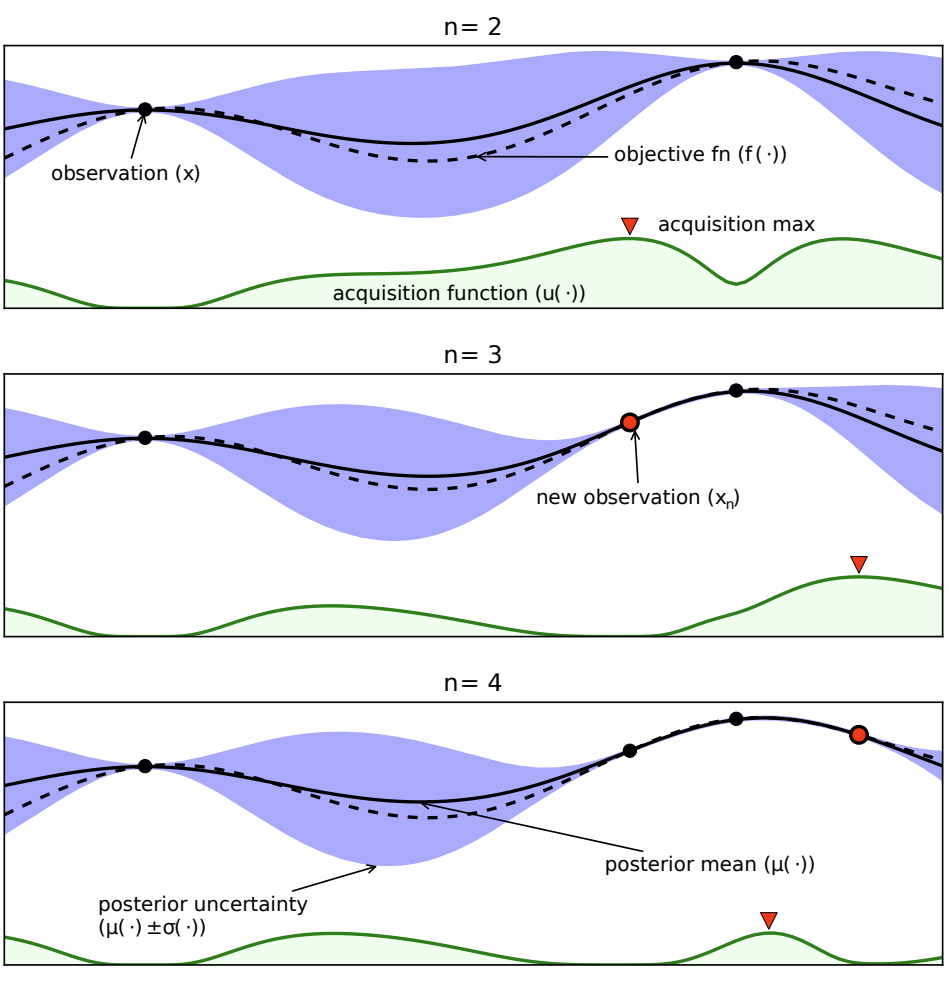
\includegraphics[width=120mm]{img/Bayes_opt.png}
  \caption{Overview of a 1-dimensional Bayesian optimization process. Image by~\citet{Bayes2016}.}
  \label{fig:bayes_opt}
\end{figure}

We used \texttt{mlrMBO} library\footnote{\url{https://mlrmbo.mlr-org.com/}} that implements Bayesian optimization and allows us to define our objective function we want to minimize. 

For the acquisition function we selected \texttt{ExpectedImprovement} mostly because it seems to perform well in most applications\cite{Bayes2016} and since we are leveraging multi-point evaluation in order to utilize multi-threading it will be its multipoint modification \texttt{q-EI}\cite{bayes_multipoint}.

In order to minimize overfitting concerns we generated four distinct data sets of 100 000 cells each, that differ in the characteristics of their strong markers - two have the same strong markers but with a different floor and two lack strong markers. Each data set also uses different random seed.

Loss is then calculated as average of mean squared errors of all three data sets after Nougad unmixing using the selected hyperparameters against their respective ground truths. We ran the model for 2000 iterations which required over 30 hours of computation time.

Note that deeper dive into Bayesian optimization, different acquisition functions and their properties is outside of the scope of this thesis. Everything needed for our application is well explained and illustrated in \cite{Bayes2016} which can also serve as a good starting point for any reader wishing to delve deeper. 

\subsection{Parameter ranges for tuning}
For \param{spw} and \param{spw} we decided to go with range of 1--300 since in preliminary testing with values up to 2000 there were no competitive results with either set over 300.

Similarly for \param{nw} we choose the ceiling of 2000 since in preliminary tests anything higher did not seem beneficial and would often lead to \texttt{NaN} results. Overall this is the parameter where we know for a fact that it must be set somewhat high to exploit the main advantage of Nougad - soft constraint for negative spectral abundances. 

For \param{start} we picked the range of 1--500 reasoning being that for our artificial data the median value after umixing and clamping to 0 using OLS, WLS or even less optimized Nougad tends to lie between 300--400 which is not far off the median value for ground truth. Setting this close to median of clamped unmixed result could work as a reasonable rule of thumb for real data as well.

We know that learning rate - \param{alpha} should not be set too high in order to avoid \texttt{NaN} results. This cutoff seems to be around 0.1 value from preliminary testing that was done in 0.001--1 range. Furthermore, values of over $0.02$ did not seem to provide competitive results overall. Range for more thorough testing was kept between 0.001--0.02 with increments of 0.001.

After some preliminary testing for \param{accel} with already established ranges for other parameters we settled on 0.001-1 with 0.001 increments. Values $> 1$ seem to produce \texttt{NaN} quite reliably when using higher values for \param{nw} (which is necessary to improve Nougad performance).

Overall there is varying degree of interplay between all parameters so their values cannot really be discussed in a vacuum (maybe with the exception of \param{start}).

Finally even though our chosen optimization strategy allows us to set continuous ranges for all the parameters we decided to not leverage this option. Mostly for simplicity, but also because there seems to be no argument as to why this option would lead to a significantly improved results. Ranges are therefore in integers with $\text{step size} = 1$ unless otherwise specified.

\subsection{Tuning outcome}
We managed to reduce mean squared error on testing data set almost two-fold when compared to manual tuning and almost four-fold when compared to default values of Nougad function (which behave indentically to OLS).

The script used for tuning (including the custom objective function and hyperparameter ranges) is available in the supplement.
 
\section{Unmixing quality metrics}
The main advantage of the simulated data is that we can objectively and easily measure the difference between the two $n \cdot m$ matrices --- the abundance matrix $U$ produced by currently evaluated unmixing algorithm and the ground truth abundance matrix $A$. Mean squared error (MSE) is perfectly suitable for this:
\[MSE=\frac{1}{nm}\sum_{i=1}^{n}\sum_{k=1}^{m}(A_{ik}-U_{ik})^2\]
In other words we are computing the mean of elementwise squared error between the two abundance matrices.

The reason we are using squared error is that emphasizes outliers and de-emphasizes small noise. Both of those things are desirable for us. We don't really mind if a cell is shifted by a fraction from its real coordinates, however big location shifts in our multidimensional space are problematic and can lead to some fundamentally incorrect conclusions. 

We will also be looking at per cell MSE, squared error distribution over the entire data set and in individual spectra and spectra pairs. Finally we leverage embedding and dimensional reduction using Self-Organazing Maps (SOM) implemented in R package EmbedSOM\cite{ESOMpap}. 

\subsection{Evaluation on real-world experimental data}

While simulated data should approximate the characteristics of real data, the truth is that no model is perfect.

As far as the author of this thesis knows no truly objective method for evaluating unmixing performance on data without known ground truth exists.

Despite this fact it is still useful to try to visualize and tentatively compare both real data from peripheral blood of a helthy patient and artificial.

\subsubsection{Comparison of artificial to real data}
Visualizations are done using UMAP assisted embedding into 2D using \texttt{EmbedSOM} library. 

First we take a look at the real and artificial data comparison. From \cref{fig:SOM_comp} we can see that clusters defined by the selected markers are present in both data sets. In artificial data there is significantly more fragmentation within these clusters which is caused by `sharply' defined phenotypes. This is not replicated in real data as some of the phenotypes are simply not present and there is even more noise for the ones that are.

\begin{figure}
  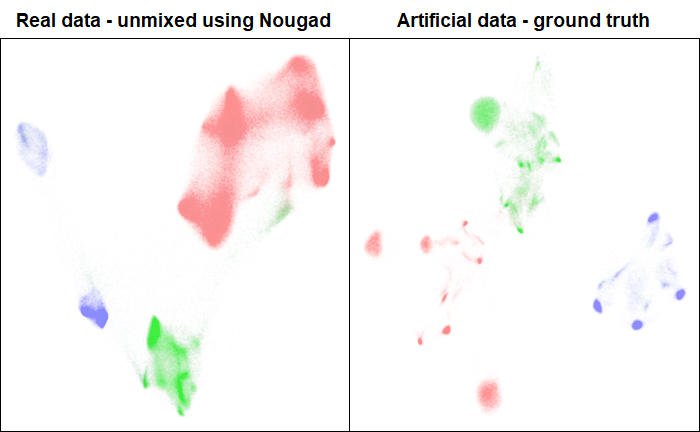
\includegraphics[width=1\linewidth]{img/SOM_comp_real_artv2.png}
  \caption{Comparison of real and artificial data --- colored by CD4 (red), CD8 (green) and CD16 (blue) markers.}
  \label{fig:SOM_comp}
\end{figure}

Ultimately there clearly are some fundamental differences between data sets however, broader structure in the artificial data seems similar enough to the real data for the purpose of unmixing method evaluation. 


\chapter{Results and discussion}

\section{Performance of alternative optimizers}
We have tested performance of nougad using the seemingly promising ADAM optimizer, which has been shown to consistently perform well for variety of different problems. 

However, in the hyperparameter tuning stage it became clear that we won't be able to match or even approach performance of the momentum-based optimizer. The problem seems to lie in the fact that a combination of $\beta_1$ and $\beta_2$ decay factors for the first and second moment and $\alpha$ learning rate, that could provide fast enough convergence for ADAM optimizer to be competitive and practical to use, leads to under/overflows and produces \texttt{NaNs}. MSE produced by the best discovered parameter set fell short even when compared to OLS.

The surprisingly lackluster performance of ADAM optimizer compared to the momentum-based method leads us to believe that evaluating alternative optimizers could prove worthwhile.

\section{Quality of the artificial datasets}

In order to examine the overall structure of the generated data we used the R package EmbedSOM\footnote{\url{https://github.com/exaexa/EmbedSOM}}, that allows us to perform dimensional reduction via embedding the data into a 2D Self-Organizing Map (SOM) guided by Uniform Manifold Approximation and Projection (UMAP) generated landmarks: \cref{fig:SOM_tps}.

We were satisfied with the results as they seem to exhibit cluster separation and noise characteristics similar to real experimental data. It is also clear that our model works as expected and generates the predefined phenotypes correctly.

\begin{figure}
  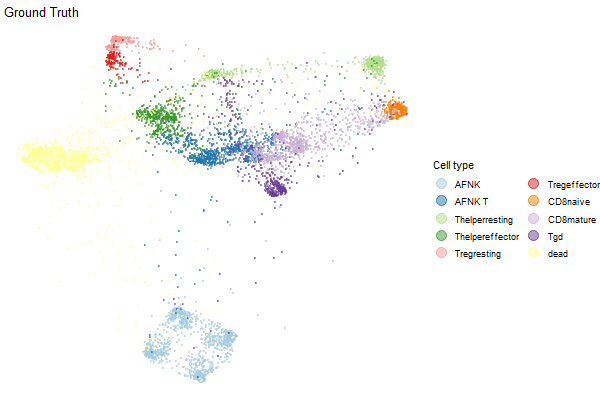
\includegraphics[width=1.0\linewidth]{img/SOM_types2.png}
  \caption{SOM embedding --- cell types in artificial data}
  \label{fig:SOM_tps}
\end{figure}

Among other manual evaluation methods we have also confirmed that our model is capable of emulating the spillover spreading artifact inherit to the process of acquisition of the real data: \cref{fig:spills}.

\begin{figure}
  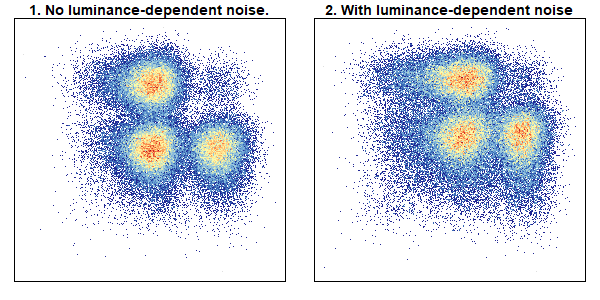
\includegraphics[width=1.0\linewidth]{img/spill.png}
  \caption{Spillover spreading simulated in the artificial data by adding fluorecent power dependent noise.}
  \label{fig:spills}
\end{figure}

\section{Quality of unmixing methods}
We are comparing three different size data sets mostly because different data size is more suitable for different types of visualizations. 
\begin{enumerate}
    \item \emph{Small data set} - $\text{size}=2002$ cells.
    \item \emph{Medium data set} - $\text{size}=10000$ cells.
    \item \emph{Big data set} - $\text{size}=100000$ cells.
\end{enumerate}

Size of the small data set is $2002$ even though the generator was passed $2000$ as the desired number of cells. This is because of previously discussed rounding - number of cells for each phenotype must be an integer. Exact sizes might change slightly if you rerun the script due to randomness.

Note that inverse hyperbolic sine transform\cite{asinh} is applied to all data sets in order to make visualizations and interpretation feasible: \cref{eq:asinh}.

\begin{equation}
\operatorname{arsinh} \frac{x}{100}=\ln (\frac{x}{100} + \sqrt{(\frac{x}{100})^2 + 1} 
\label{eq:asinh}
\end{equation}

The entire data generation and analysis pipeline is available as part of the supplemental materials.

\subsection{Comparison of MSE}

Mean squared errors for the testing data sets are illustrated in \cref{tab:MSEtb}.

\begin{table}[]
\begin{tabular}{lcccccc} \toprule 
\multirow{3}{*}{Method}  & \multicolumn{6}{c}{MSE}\\ 
\cmidrule(l{.5em}r{.5em}){2-7}
{}& \multicolumn{3}{c}{Unclamped}& \multicolumn{3}{c}{Clamped}\\
\cmidrule(l{.5em}r{.5em}){2-4}
\cmidrule(l{.5em}r{.5em}){5-7}
{} & small & medium & big  & small   & medium   & big\\
\midrule
\textbf{Nougad} & 0.5558  & 0.5452 & 0.5433 & \textcolor{red}{0.4942} & \textcolor{red}{0.4875}  & \textcolor{red}{0.4871}  \\
\textbf{WLS} & 2.1315 & 2.1795  & 2.1907  & 0.7752   & 0.7827 & 0.7833 \\
\textbf{OLS} & 1.9856  & 2.0197 & 2.0387  & 0.7337   & 0.7393 & 0.7417 \\
\bottomrule
\end{tabular}
\label{tab:MSEtb}
\caption{MSE on testing data sets across all methods.}
\end{table}

It is immediately obvious how much does simply clamping the results to zero help for OLS and WLS methods and while it helps for Nougad the difference is rather small. This does however, make some sense. There is no such thing as negative expression but OLS and WLS do not have any non negative constraints therefore shifting the negative results to zero must decrease the error. Same thing applies for Nougad however since this algorithm is already heavily biased towards positive results thanks to high \param{nw} parameter the difference is rather small. 

Nougad clearly comes out on top in this comparison. However, OLS performs quite well when clamped to zero and we could say it gets close to Nougad while WLS performs the worst out of the three, both clamped and unclamped.

Hypothesis testing using squared error was done to verify than Nougad outperforms both competing methods (clamped and unclamped) with statisticall significance.

\subsection{Distribution of errors in the result}
Calculated and visualized on big data set.


In this section we examine the distribution of squared errors across the entire data set. Since this is per element error even the smallest data set is almost too large for this visualization giving us $2002\cdot21=42042$ points. 

From \cref{fig:SE_auc} is evident that when we are comparing the unclamped results there is no contest Nougad clearly performs the best.

\begin{figure}
  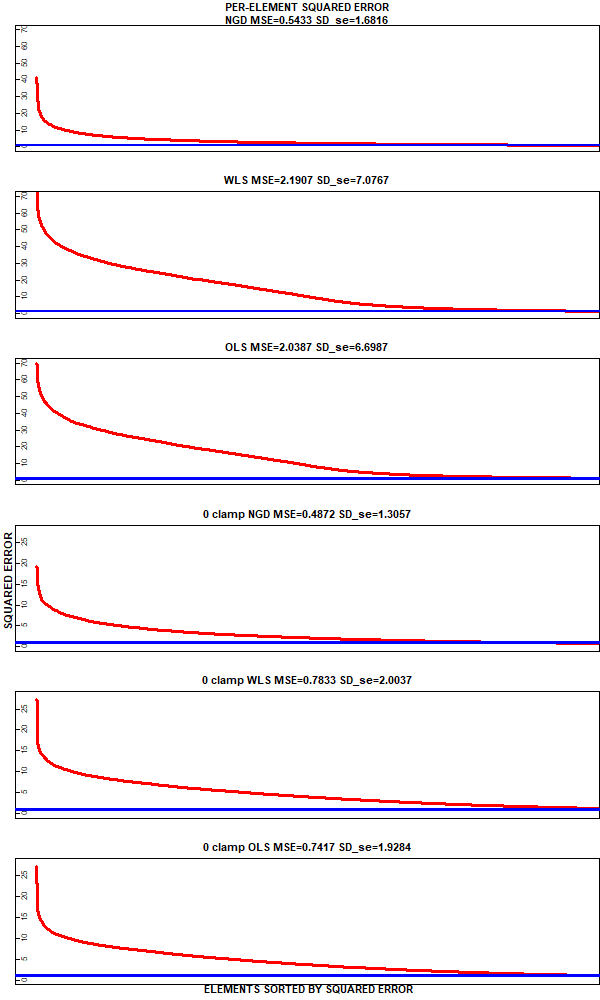
\includegraphics[width=0.9\linewidth]{img/SE_auc.png}
  \caption{Per-element squared error for individual data sets sorted from highest --- blue line represents SE=1.}
  \label{fig:SE_auc}
\end{figure}

Clamping the methods results in significantly reduced error especially for OLS and WLS. What is quite interesting is that the top error percentile has decreased significantly for both linear methods as well. This suggests that the biggest errors produced by these methods stem from negative abundances. Still Nougad remains in the even compared to clamped OLS.

\subsection{Per-cell mean squared error distribution}

Calculated on big data set, visualized on small data set.

This comparison focuses on per-cell MSE represented by the red line, while the green line denotes relative luminance of the given cell. Vertical labels for cell types are also added: \cref{fig:MSEcell_dist}.

When unclamped similarly to the previous sections Nougad is clearly superior to both OLS and WLS. It is interesting to note that while there seems to be a degree of correlation between cell luminance and absolute MSE value, it does not appear as strong as we would perhaps expect and seems even weaker in the data unmixed by Nougad compared to the other two methods.

\begin{figure}
  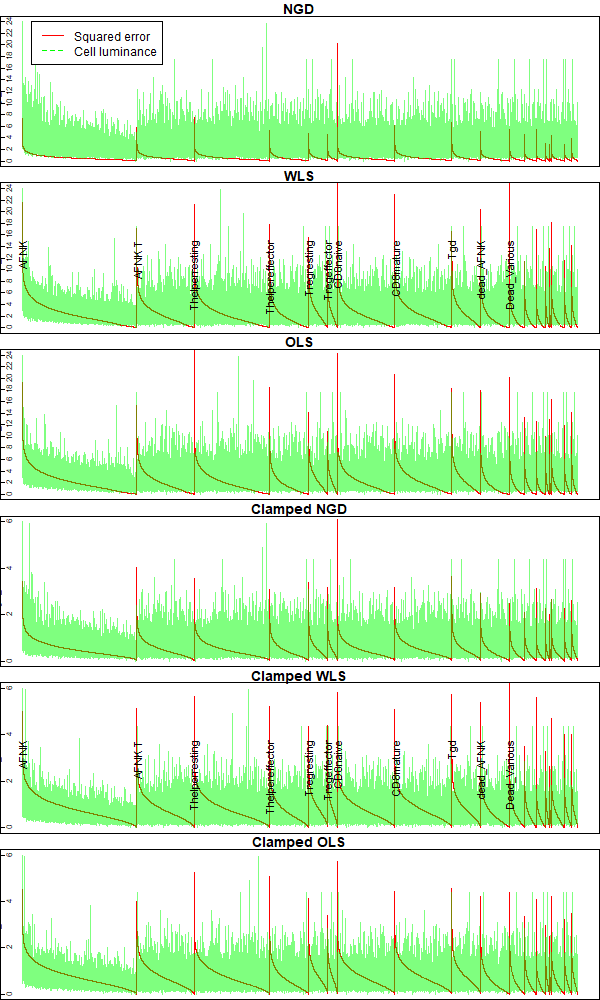
\includegraphics[width=1.0\linewidth]{img/errdist.png}
  \caption{Per-cell MSE distribution using unclamped methods}
  \label{fig:MSEcell_dist}
\end{figure}

After clamping the methods we can see that OLS performs much closer to Nougad, but Nougad still retains the overall advantage.

\subsection{Correlation of unmixing error with cell luminance}

The idea behind this metric is that the better the unmixing method is, the more it should avoid increasing the absolute error proportionally to the cell luminance.  

Nougad shows significantly lower correlation than other methods both clamped and unclamped: \cref{fig:bright_cell_cor}. Correlation for nougad could be condidered borderline weak while for other methods it lies firmly in the moderate territory\cite{cor2018}. This suggests that nougad is better equipped to deal with the luminance-dependent noise.

\begin{figure}
  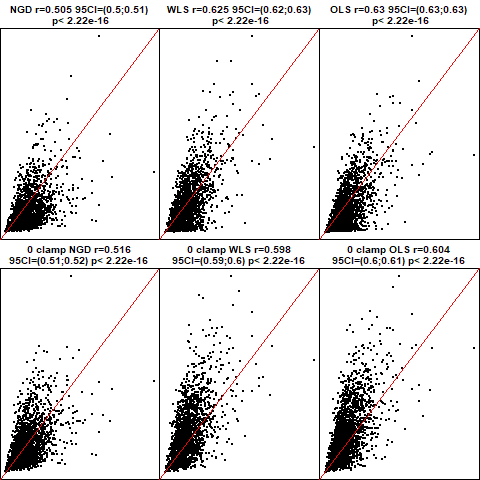
\includegraphics[width=0.8\linewidth]{img/lumcorr.png}
  \caption{Correlation of per-cell MSE with cell luminance}
  \label{fig:bright_cell_cor}
\end{figure}

\subsection{Error distribution in individual dimensions}


This metric focuses on unmixing performance over individual spectra.

On per-spectrum basis there are some instances where the difference betwenn nougad and investigated linear methods is quite small. One such case is the spectrum for the CD4 marker when unmixing using clamped methods : \cref{fig:hists}(b). However, even though the performance of clamped linear methods can get quite close to that of nougad, this is more of an exception than a rule. Overall nougad outperforms both OLS and WLS across most of the spectra.


\begin{figure}
  \centering
  \subfloat[][]{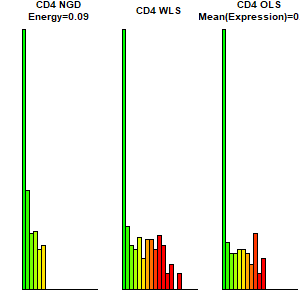
\includegraphics[width=.45\linewidth]{img/CD4.png}}\quad
  \subfloat[][]{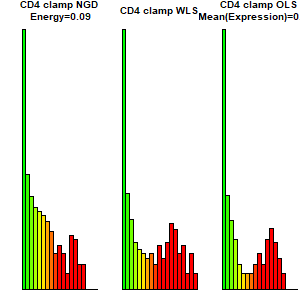
\includegraphics[width=.45\linewidth]{img/CD4_clp.png}}\\
  \subfloat[][]{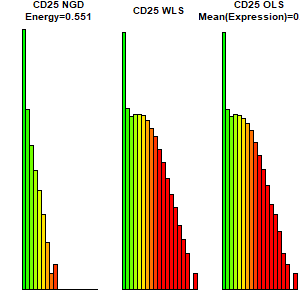
\includegraphics[width=.45\linewidth]{img/CD25.png}}\quad
  \subfloat[][]{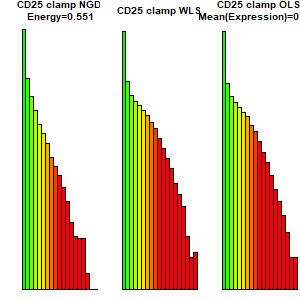
\includegraphics[width=.45\linewidth]{img/CD25_clp.png}}
  \caption{Histograms of per-cell MSEs for CD4 and CD25 antigens. Caution --- bin width and x limits differ between clamped and unclamped methods!}
  \label{fig:hists}
\end{figure}

It is important to highlight that the X axis limits and therefore bin width differ between clamped and unclamped comparisons which means that we cannot directly cross-compare the two. However, relative comparisons are of course completely valid.

Also note that the histograms are log-scaled and the first bin is always clipped.

This metric was calculated and visualized on the big data set. Histograms for all remaining spectra can be found in the supplement.

\subsubsection{Per-spectrum MSE correlation with luminance}

Intuitively we would expect higher error in dimmer spectra but the analysis is inconclusive as confidence intervals are too wide and there is no statistically significant difference between methods.

Calculation performed on the big data set with exact results including $95\%$ CIs and p-values can be found in the supplement.

\subsubsection{Per-spectrum mean error correlation with average expression}

Our analysis supports the hypothesis that mean per-spectrum SE is inversely correlated with mean expression. The results suggest medium to strong inverse correlation across all methods clamped and unclamped. Confidence intervals are very wide therefore, there is no statistically significant difference between individual methods.

Calculation performed on the big data set with exact results including $95\%$ CIs and p-values can be found in the supplement.

\section{Observing the detailed errors on dot-plots}

This comparison gives more insight into how much is the cell's position in some of the sub-spaces given by spectra pairs affected by errors.

Black points represent the ground truth --- cell's original location in the selected 2D subspace while red lines are drawn from this point to the location of the same cell in the unmixing result for the examined method. This metric is visualized on the big data set.

Looking at some of the markers the difference can be quite small even in unclamped methods as demonstrated in \cref{fig:bld}(b), where it could even be argued that OLS slightly outperforms nougad. However, this is again more of an exception as nougad has a clear advantage in most other, both stronger and weaker markers, as exhibited in \cref{fig:bld}(a,c,d). An argument could be made for OLS outperforming WLS.

\begin{figure}
  \centering
  \subfloat[][]{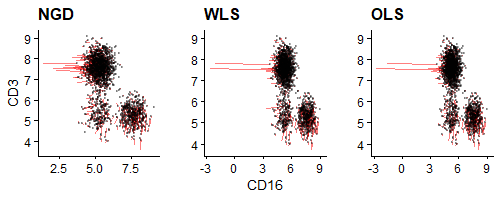
\includegraphics[width=0.7\linewidth]{img/blood_CD16xCD3_nocl.png}}\\
  \subfloat[][]{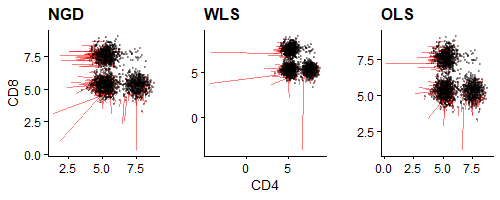
\includegraphics[width=0.7\linewidth]{img/blood_CD4xCD8_nocl.png}}\\
  \subfloat[][]{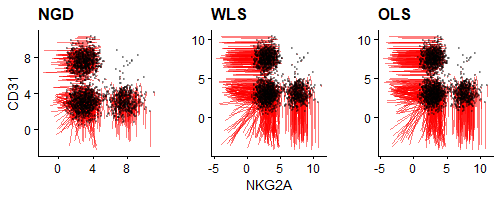
\includegraphics[width=0.7\linewidth]{img/blood_NKG2AxCD31_nocl.png}}\\
  \subfloat[][]{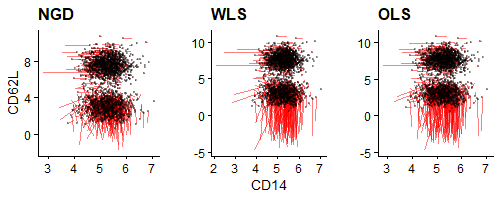
\includegraphics[width=0.7\linewidth]{img/blood_CD14xCD62L_nocl.png}}
  \caption{2D plots on selected markers for unclamped methods.}
  \label{fig:bld}
\end{figure}




\begin{figure}
  \centering
  \subfloat[][]{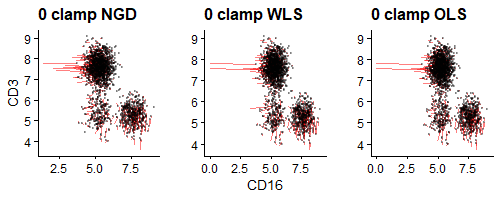
\includegraphics[width=0.7\linewidth]{img/bloodCD16xCD3_cl.png}}\\
  \subfloat[][]{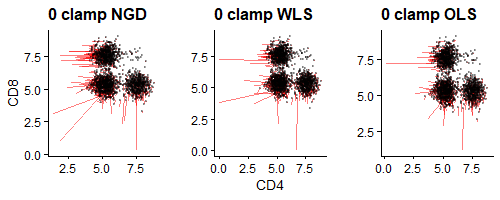
\includegraphics[width=0.7\linewidth]{img/bloodCD4xCD8_cl.png}}\\
  \subfloat[][]{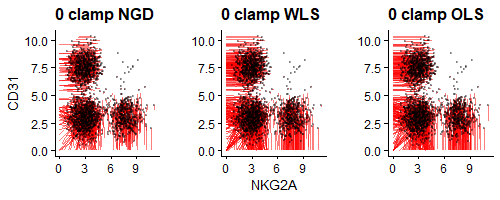
\includegraphics[width=0.7\linewidth]{img/bloodNKG2AxCD31_cl.png}}\\
  \subfloat[][]{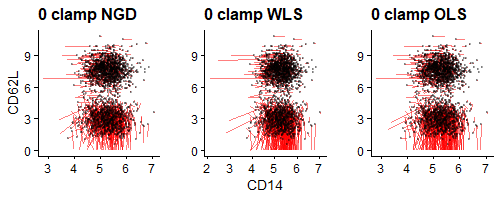
\includegraphics[width=0.7\linewidth]{img/bloodCD14xCD62L_cl.png}}
  \caption{2D plots on selected markers for clamped methods.}
  \label{fig:bld_cl}
\end{figure}

When we examine the clamped methods, OLS, WLS and nougad seem to trade blows more often than previously. However, nougad still wins in most comparisons \cref{fig:bld_cl}.

We have prepared another type of visualization for the same data --- plotting the ground truth and unmixing results for each of the three methods as separate plots and color the points by the severity of the error.

This type of visualization helps to emphasize the fact that the majority of the more severe errors tends to happen in the weaker markers.

Main advantage of Nougad is well illustrated in \cref{fig:blob_noclp} and \cref{fig:blob_clp} where we can see that just clamping the method and effectively putting all negative points onto an axis is not an optimal solution and even though the difference in error might not be that big the way Nougad deals with such situations is clearly superior. 

\begin{figure}
  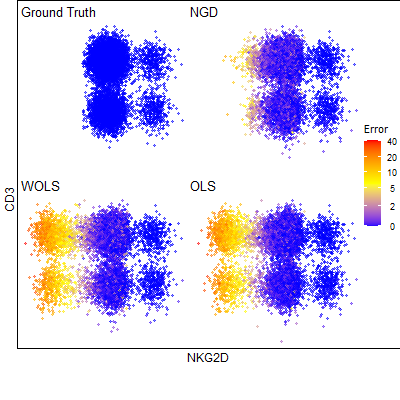
\includegraphics[width=0.7\linewidth]{img/blobs_noclp.png}
  \caption{2D error color plot NKG2D$\times$CD3 unclamped}
  \label{fig:blob_noclp}
\end{figure}

\begin{figure}
  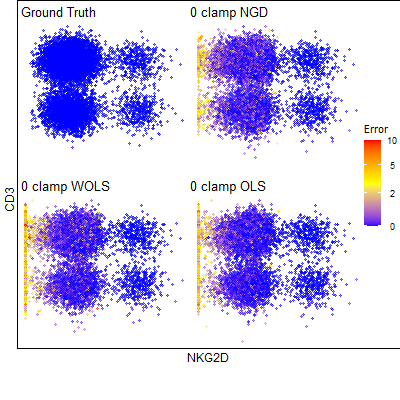
\includegraphics[width=0.7\linewidth]{img/blobs_clp.png}
  \caption{2D error color plot NKG2D$\times$CD3 clamped}
  \label{fig:blob_clp}
\end{figure}

2D plots of both types for all unique spectra are available in the supplement. 

\section{Error overview using dimensionality reduction}
In order to further examine the per-cell error characteristics in all dimensions we used the previously generated UMAP guided SOM from \cref{fig:SOM_tps} for 2D visualization. Unmixing results for the evaluated methods are embedded into the SOM and colored by per-cell MSE.

As evident from \cref{fig:SOM_noclp} Nougad takes a comfortable lead against unclamped methods. 

\begin{figure}
  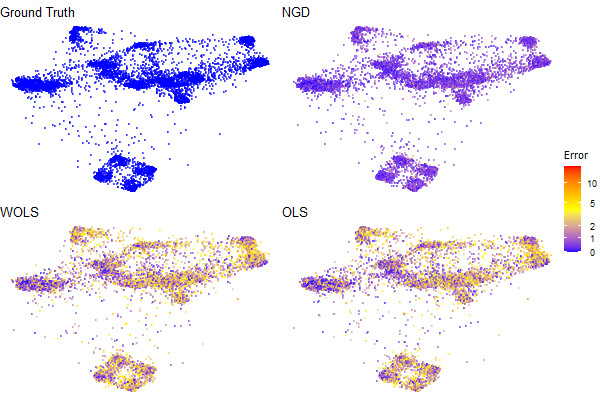
\includegraphics[width=1.0\linewidth]{img/SOM_err_noclp2.png}
  \caption{SOM embedding colored by MSE unclamped}
  \label{fig:SOM_noclp}
\end{figure}

When clamped the differences between Nougad and OLS become much harder to spot as they are practically interchangeable: \cref{fig:SOM_clp}. 

\begin{figure}
  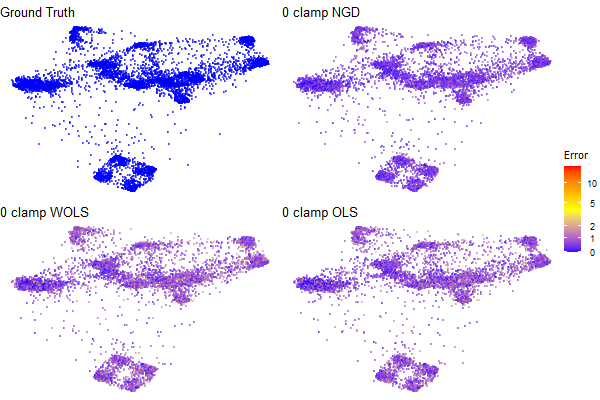
\includegraphics[width=1.0\linewidth]{img/SOM_err_clp2.png}
  \caption{SOM embedding colored by MSE clamped}
  \label{fig:SOM_clp}
\end{figure}

Finally we can take a look at the different unmixing methods and their comparison to ground truth using the `blood plots'. Do note that we did have to increase expression based and luminance based noise when generating the data for this visualization in order to make the differences more apparent to the reader. Arguably this is more true to life, since real data do tend to be quite noisy. 

\begin{figure}
  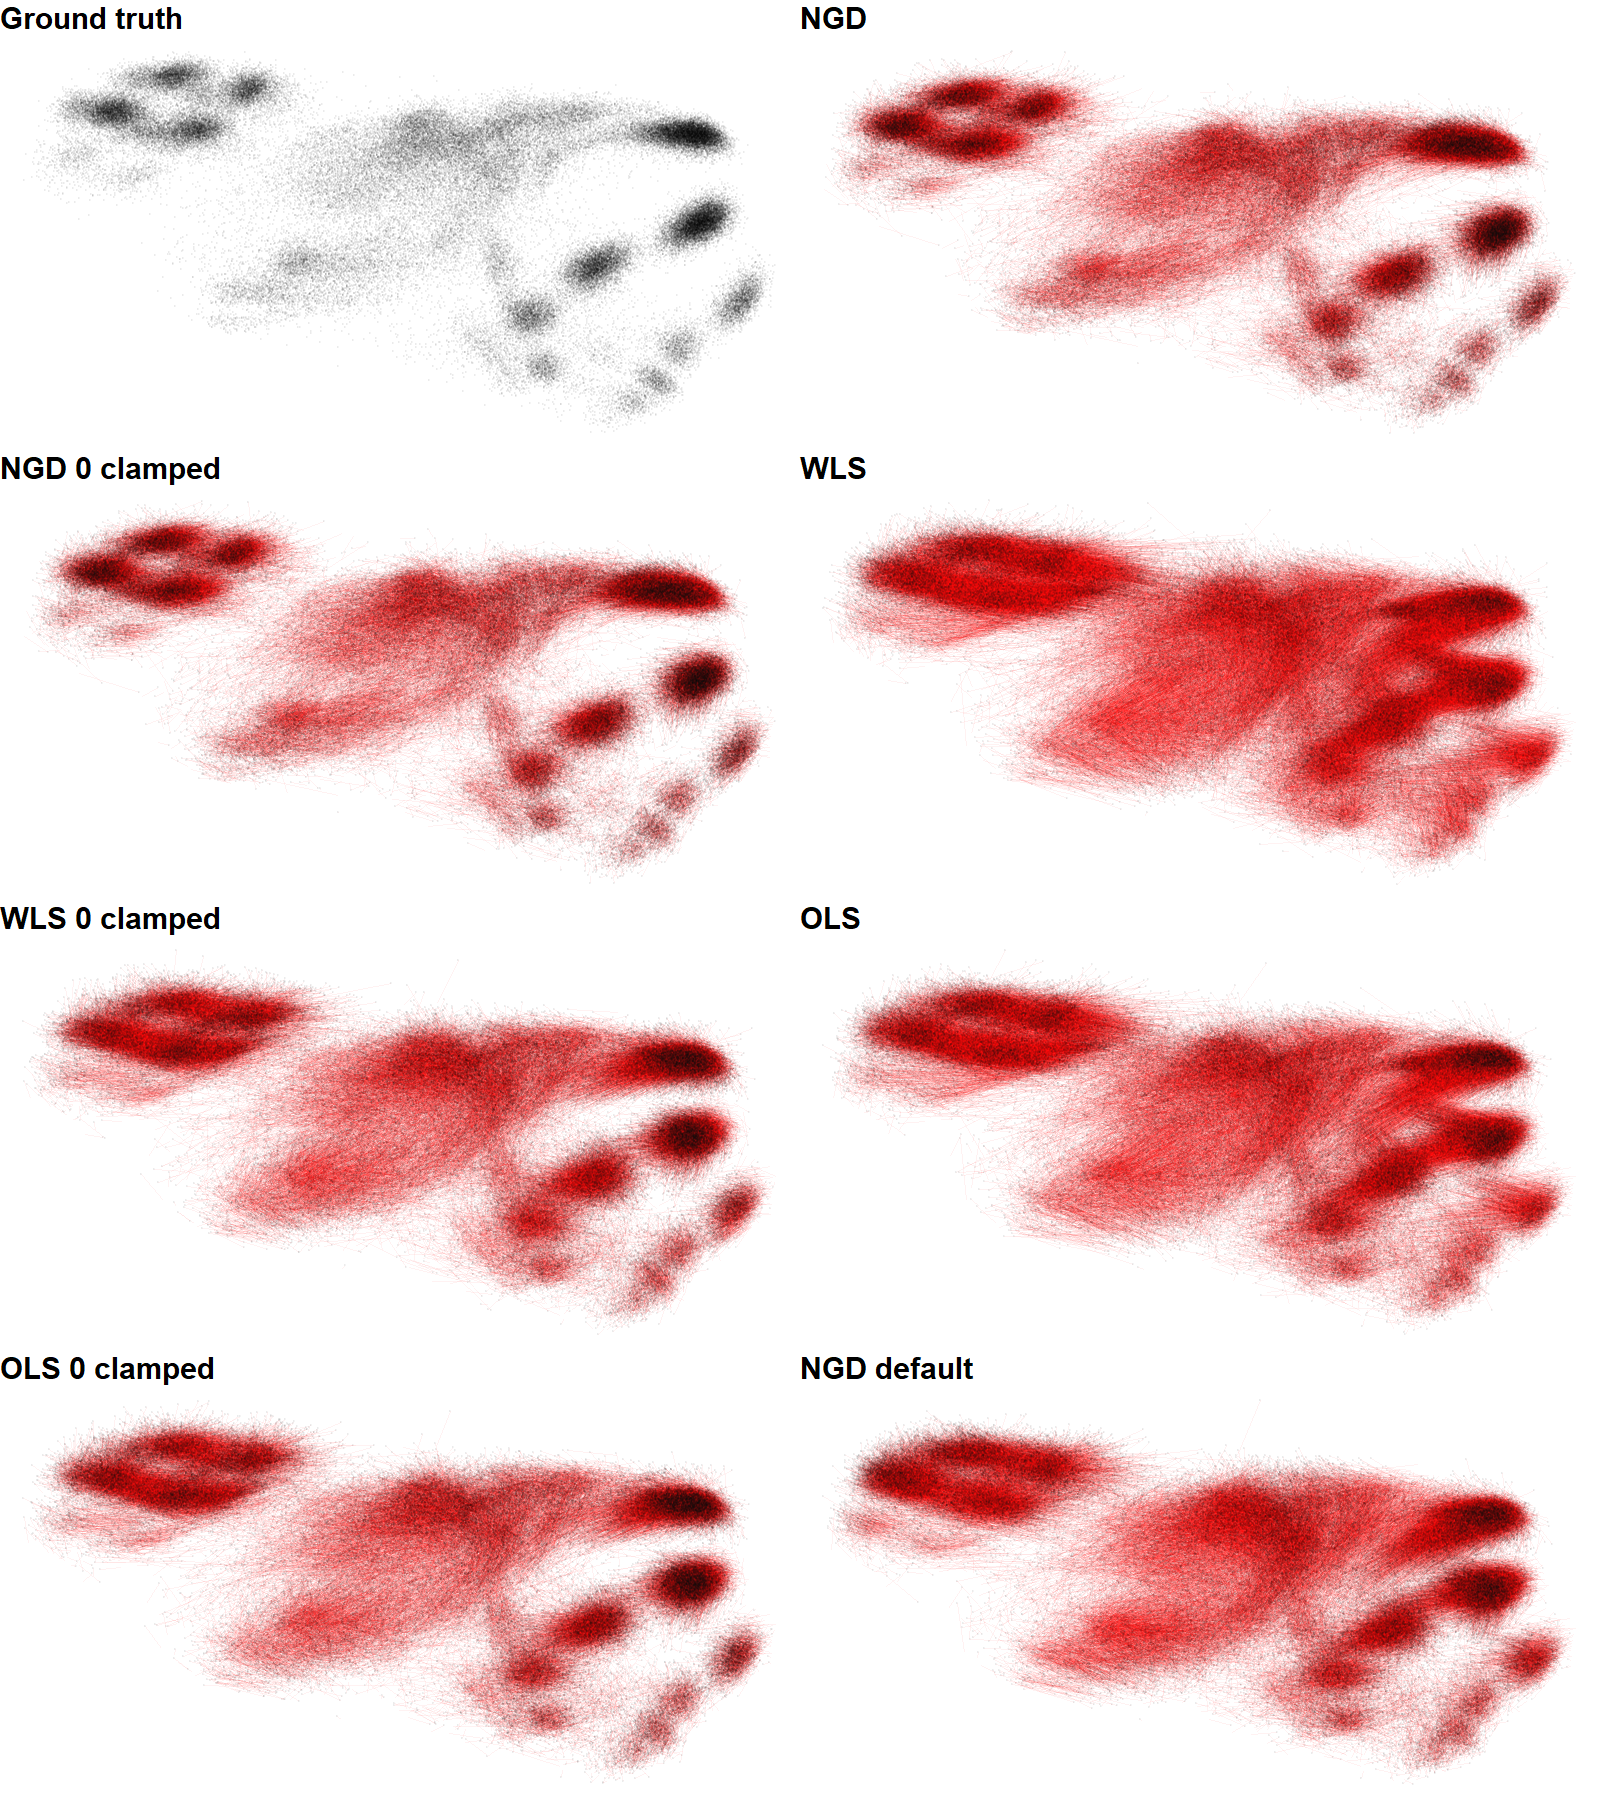
\includegraphics[width=1\linewidth]{img/8-way.png}
  \caption{Error comparison for investigated unmixing methods in 2D using SOM embedding.}
  \label{fig:8-way}
\end{figure}

Note that in \cref{fig:8-way} we are using `inverse blood plots' --- the black/grey points are drawn in the location of unmixed data and red lines are drawn from those points towards the ground truth location. This is done to improve readability and make easier for the reader to spot the differences. That said, this plot can be interpreted in a similar way as previous blood plots --- more red lines means more errors. This comparison clearly shows that Nougad performs the best with previously established hierarchy for the remaining methods. Nougad tends to most faithfully retain the cluster separation which is a challenge for all other methods and while clamped OLS gets somewhat close the difference is still clear. We also choose this visualization to demonstrate that hyperparameter tuning clearly matters --- Nougad with default parameters performs somewhat similarly to clamped WLS, meaning clearly better than unclamped WLS and OLS and clearly worse than clamped OLS and therefore significantly worse than Nougad with optimized hyperparameters.
Size of both data sets used for visualization was $\sim$100 000.

\section{Results on real-world datasets}
While we cannot evaluate how well the different methods perform on a real data set, since the ground truth is not known, we can still do a relative comparison and comment on the differences.

\begin{figure}
  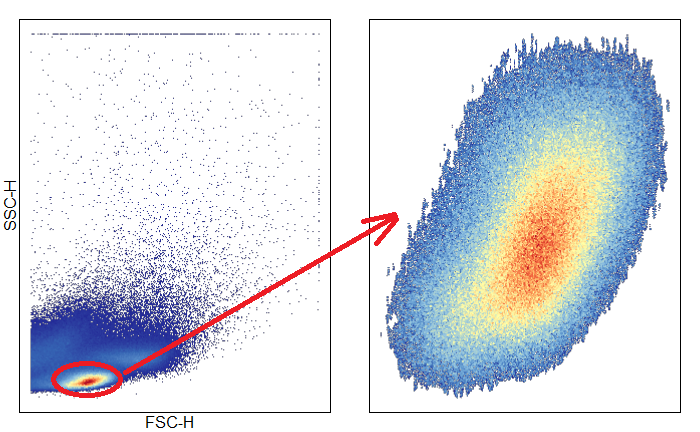
\includegraphics[width=1\linewidth]{img/my_gate.png}
  \caption{Isolating Lymphocytes from the experimental data set using density-based gating approach (Lymphocyte population circled red).}
  \label{fig:my_gate}
\end{figure}


We will limit our comparison to Lymphocytes to remain consistent with the artificial data. Our gating strategy is visualized in \cref{fig:my_gate}. Note that we decided to forgo the more traditional manual gating strategy in favor of density-based gating using k-nearest neighbors algorithm that allows us to isolate high density regions and their neighborhood (implementation available in the supplement).

In \cref{fig:6-way_nb} we can see how the spatial organization of real data looks after unmixing when embedded --- the data is colored using selected markers.

There are no truly objective conclusions to be drawn here. Only thing we can be fairly certain about is that relative differences between methods are somewhat consistent with the artificial data. Nougad in both its variations is the most dissimilar to the other methods while its variants seem quite close to each other. Both OLS and WLS differ quite a bit between their clamped and unclamped versions and we could argue that OLS in its clamped variation is the least dissimilar to Nougad out of all OLS and WLS variants. Note that due to the nature of the algorithm used for embedding and plot generation there is no good way to force the same orientation of the resulting maps however it should be fairly obvious which clusters correspond to each other in maps for different methods.

We must stress that this comparison is purely empirical and somewhat subjective therefore it should not be used to draw any conclusions about the performance of these algorithms.

\begin{figure}
  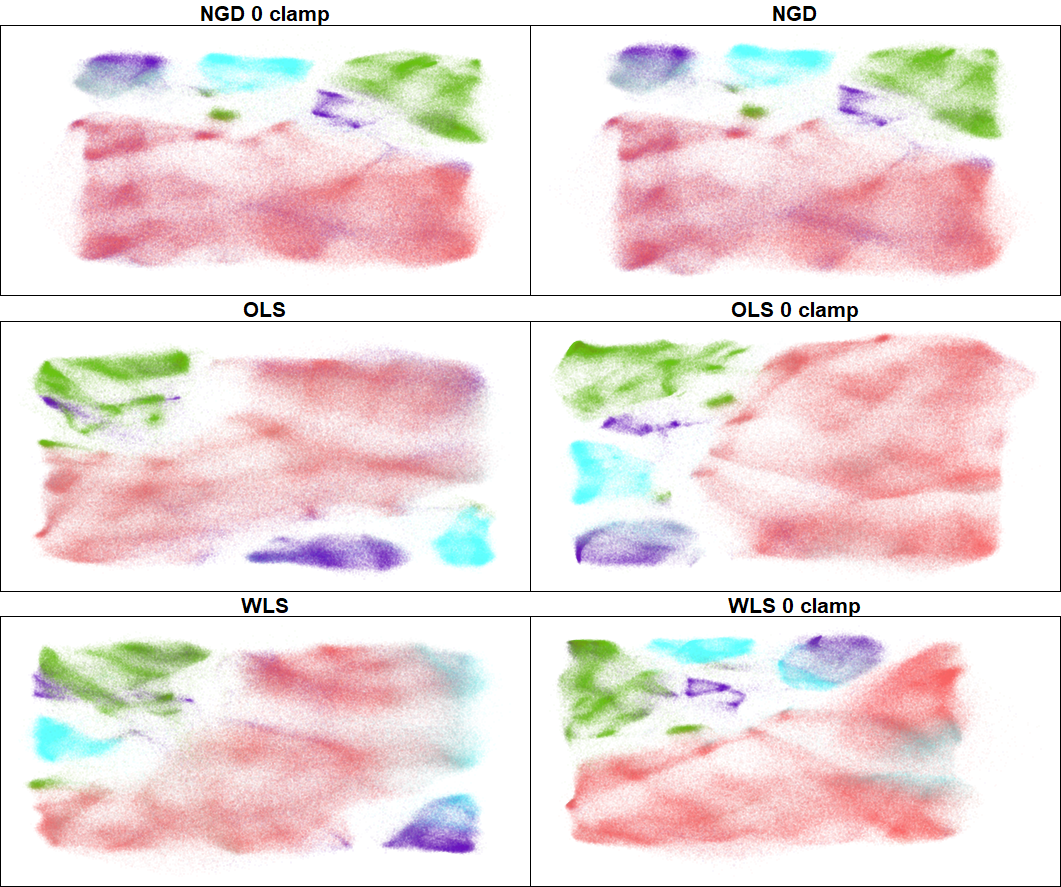
\includegraphics[width=1\linewidth]{img/6way_asinh1000v2.png}
  \caption{Real data unmixed via tested methods visualized in 2D using SOM embedding. Colored by selected markers --- CD4 (red), CD8 (green), CD16 (cyan) and gdTCR (blue).}
  \label{fig:6-way_nb}
\end{figure}

\section{Discussion}
We have found that for our simulated data Nougad algorithm consistently performs better than OLS and WLS alternatives, both clamped and unclamped. While there is a possibility than in some instances in low-error regions Nougad could be outperformed by clamped OLS, this is more of an exception than a rule. Furthemore, in medium or high-error regions Nougad, even in its unclamped variation, significantly outperforms clamped OLS. In our opinion potentially getting slightly more noise in a low-error region seems like a worthwhile trade-off for consistently better handling of more challenging regions.  

Results show that for the tested artificial data Nougad is the better choice. 

The validity of the simulated data cannot be entirely proven however, it should be sufficient for the evaluation of unmixing performance.

Objective performance evalution for different unmixing methods is not possible on real experimental data which is why we do not consider provided real data comparisons to be evaluation metrics. We do however make an argument that the relative differences between the methods seem to hold even in real data.

Ultimately our testing is limited --- we cannot guarantee same performance across all possible experiment types, hardware configurations and other variables. On the other hand there is nothing that would lead us to believe that Nougad should fail for data with different characteristics (within reason of course). Another limitation is the reliance on optimized hyperparameters --- it is possible that for significantly different combinations of fluorochromes and detectors the optimal hyperparameters will differ. Of course since our tuning process is well documented and reproducible it is possible to replicate it for different conditions. 

As a result we do believe that Nougad provides a viable and likely superior alternative to OLS and WLS for unmixing of spectral flow cytometry data, especially for those who would like to avoid using `black box' and usually paid software provided by different private companies. We would therefore recommend considering Nougad as unmixing algorithm of choice to scientists who value maximum reproducibility and transparency for their experiments.
\chapwithtoc{Conclusion}

The main goal of this thesis was to evaluate the performance of a non-linear unmixing algorithm nougad, and compare it to two commonly used linear alternatives --- ordinary and weighted least squares unmixing. 

To objectively measure the performance, we implemented a data-generating pipeline that simulates common phenomena in cytometry measurements, enabling us to generate artificial data with known ground truth that are sufficiently similar to realistic datasets. The model reproduces the common cell distributions and several phenomena caused by measurement noise, such as spillover spread.

A detailed performance comparison and evaluation of the tested method is the main result of this thesis. We provided both numeric and visual comparisons and highlighted the main differences, exploring their possible causes. Because of the need for ground truth in datasets, this comparison is inherently limited to simulated datasets (as it is currently nearly impossible to obtain sufficiently detailed ground truth for real cytometry data). For empirical illustration, we additionally showed how the algorithm differences impact the outcome on an example whole-blood dataset from a real experiment.

As a side result, we improved the nougad algorithm by providing a simple multi-threaded implementation that computes the results faster. We additionally tuned the algorithm hyperparameters using Bayesian optimization, obtaining an improvement in the testing metrics.

While we did not find the ultimate solution to the unmixing problem in spectral flow cytometry, we have created an evaluation methodology that can be used to scrutinize and optimize the possible upcoming algorithms. As a main outcome, it seems that the non-linear unmixing based on algorithms similar to nougad is a very promising choice for the future of cytometry, and should be considered for future research and experiments.

\section*{Future Work}

It is possible to further tune the model used for generating the artificial data. Here multiple different approaches could be taken including introducing even more variables and modelling more than two noise sources. In order to find optimal values for the various hyperparameters Expectation-maximization approach seems like the best fit and given enough time and resources it is worth exploring. Also simulating cell types other than just Lymphocytes (such as Monoctyes, Macrophages etc.) could prove worthwhile.

More extensive hyperparameter tuning for Nougad itself could be performed by performing more iterations of the Bayesian search algorithm, however this would bring minor performance improvement at best. 

It would also be beneficial to test the algorithms on data generated using spectra from measured on different instruments using different number detectors with various configurations and different fluorochromes. We are also positive that there are other metrics that are relevant and could be used to extend our evaluation. 

Finally some type of objective evaluation on real data would be most desirable but most likely impossible. However, an empirical evaluation by multiple experts in the field would likely be beneficial. 


\ifEN
\chapwithtoc{Bibliography}
\else
\chapwithtoc{Seznam použité literatury}
\fi

\printbibliography[heading=none]


\appendix
\chapter{Using R scripts and markdown files}

This appendix serves as a very concise guide to supplemental materials.

To compile and run the scripts and Markdown document, you will need R (preferably in the latest version). You will also need to install all the libraries that are loaded at the start of scripts/markdowns.

Non-standard libraries:
\begin{itemize}
    \item My implementation of \texttt{multithreaded nougad} is available from: \url{https://github.com/mattejn/nougad_mt}.
    \item Original \texttt{nougad} from: \url{https://github.com/exaexa/nougad}.
    \item And \texttt{EmbedSOM} package from: \url{https://github.com/exaexa/EmbedSOM}.
    \item The materials themselves can be downloaded from GitHub as well: \url{https://github.com/mattejn/artificial_data_comp/}.
\end{itemize}

All other libraries should be available from standard repositories. 

The supplement folder for this thesis contains 5 files:

\begin{enumerate}
    \item \textbf{Main markdown file:} \begin{verbatim}`Appendix.Rmd'\end{verbatim}
    
    A notebook in R markdown format containing scripts responsible for artificial data generation, numerical comparisons and the vast majority of visualizations used in this thesis (including a lot of unused). Comments headings and short descriptions should make the function of each chunk apparent. Keep in mind that executing some of the functions, such as data generation and unmixing or Extensive plotting/embedding on thousands of points and sometimes up to hundreds of plots can be quite computationally expensive and take a long time. 
    
    \item \textbf{Function file:} \begin{verbatim}`functions.R'\end{verbatim}
    
    File housing the custom functions, such as the model used to generate the artificial data and a function that builds data set objects with precalculated metrics for the main markdown file.
    
    \item \textbf{R file:} \begin{verbatim}`bayes.R'\end{verbatim}
    
    The Bayesian optimization script for hyperparameter tuning using multithreaded nougad with exact same settings and inputs as used and described for this thesis. Be aware that this will take a very long time. The optimization is set to run for 2000 iterations which, even on my quite powerful modern computer took around 30 hours. You can try and lower the number of iterations that is being passed to the `MBOControl' object. This of course no longer corresponds to the process used in this thesis.
    
    \item \textbf{A comma-separated values (csv) file:} \begin{verbatim}`phenotypes_noAFonly.csv'\end{verbatim}
    
    The phenotype table used for artificial data generation. It's characteristics are detailed in this thesis.
    
    \item \textbf{A Java-script object notation (json) file:} \begin{verbatim}`panel1_lymph_subtracted_fixed.json'\end{verbatim}
    
    The single stain Spectra used for the artificial data generator as well as unmixing of artificial and real data. Measured using the \texttt{PanelBuildeR} package with subtracted Autofluorescence.
    
\end{enumerate}

What is not included is the script used to produce visualizations containing the real data as well as \cref{fig:6-way_nb}. The real date itself is also not included. These items will be provided if requested but should not be publicly available.

% if your attachments are complicated, describe them in a separate appendix
%\include{attachments}

\openright
\end{document}
